% !TEX root = main.tex
% BMC Medical Informatics and Decision Making submission manuscript.
% Prepared with the Springer Nature sn-jnl LaTeX template.

\documentclass[pdflatex,sn-vancouver-num]{sn-jnl}

\usepackage{graphicx}
\usepackage{multirow}
\usepackage{amsmath,amssymb,amsfonts}
\usepackage{amsthm}
\usepackage[title]{appendix}
\usepackage{xcolor}
\usepackage{textcomp}
\usepackage{manyfoot}
\usepackage{booktabs}
\usepackage{url}

\graphicspath{{figures/}}

\raggedbottom

\begin{document}

\title[Self-supervised maternal comorbidity phenotyping]{Full-scale self-supervised maternal comorbidity phenotyping and cross-registry stress-testing in public birth records}

\author[1]{\fnm{Fengshang} \sur{Yan}}\email{342082145@qq.com}
\equalcont{These authors contributed equally to this work.}

\author[1]{\fnm{Qianqian} \sur{Yang}}\email{yangqianqian8733@163.com}
\equalcont{These authors contributed equally to this work.}

\author[1]{\fnm{Mingtang} \sur{Wang}}\email{1099529466@qq.com}
\equalcont{These authors contributed equally to this work.}

\author*[1]{\fnm{Feifan} \sur{Lu}}\email{luff94@163.com}

\affil*[1]{\orgdiv{Department of Obstetrics and Gynecology}, \orgname{Changhai Hospital, Naval Medical University}, \orgaddress{\postcode{200433}, \state{Shanghai}, \country{China}}}

\abstract{\textbf{Background:} Maternal comorbidity patterns are associated with adverse maternal and neonatal outcomes, but many obstetric risk models rely on private electronic health record data or supervised feature engineering. We assessed whether public birth-registry data can support reproducible self-supervised learning (SSL), phenotype discovery, and calibrated risk enrichment.

\textbf{Methods:} We used U.S. CDC/NCHS Natality records from 2016--2024. Records from 2016--2022 were used for supervised training and SSL pretraining, 2023 for development and calibration, and 2024 for temporal testing. A masked tabular transformer was pretrained on 26,345,765 records using categorical and numeric reconstruction. The fixed encoder generated 48-dimensional embeddings for 3,605,081 development records and 3,638,436 temporal-test records. Phenotype centroids were fit on 2023 embeddings and applied to 2024 embeddings. Primary endpoints were maternal core morbidity and a severe neonatal composite that excluded neonatal intensive care unit admission. Fixed phenotypes were also evaluated in linked birth/infant death records, and the workflow was rebuilt in Brazil SINASC records as an independent registry stress-test.

\textbf{Results:} A three-phenotype solution selected on all 2023 embeddings was stable across capped development-set resampling (median adjusted Rand index, 0.997; normalized mutual information, 0.991). In 2024 testing, phenotype 0 had severe neonatal outcome of 8.249\%. All-input LightGBM remained the strongest pure predictor for severe neonatal outcome (AUPRC, 0.301), whereas SSL embeddings alone achieved AUPRC 0.218 and adding SSL to all supervised inputs did not materially improve AUPRC. In 3,596,017 linked births, phenotype 0 contained 4.58\% of births and captured 16.85\% of infant deaths, whereas a transferred all-input LightGBM severe-neonatal score selected at the same fraction captured 49.09\%. In SINASC, SSL embeddings retained risk-enrichment signal but were weaker than LightGBM.

\textbf{Conclusions:} Full-scale masked tabular SSL on public birth records produced stable maternal comorbidity embeddings and phenotypes associated with adverse outcomes and linked infant death. The approach is best viewed as a reproducible public-data representation-learning and risk-enrichment framework, not as a replacement for strong supervised models or a deployment-ready clinical system.}

\keywords{Natality, SINASC, self-supervised learning, maternal morbidity, neonatal risk, phenotype discovery, calibration, public-use data, obstetric informatics}

\maketitle

\section{Background}\label{sec:background}

Maternal comorbidity and obstetric risk increasingly require models that can summarize many interacting maternal, pregnancy, and delivery-related characteristics. Diabetes, hypertensive disorders, obesity, smoking, infections, prior obstetric history, and infertility-treatment variables may combine in ways that are not fully captured by simple univariate risk strata. At the same time, clinically useful risk modeling requires transparent validation, calibration, and careful handling of rare outcomes \cite{vancalster2019calibration,saito2015precision,guo2017calibration}.

Recent high-impact obstetric informatics studies illustrate the value of reconstructing pregnancy trajectories from electronic health records (EHRs). Machine-learning models built from routinely collected EHR pregnancy journeys have improved preeclampsia risk prediction across antepartum, intrapartum, and postpartum windows, and externally validated EHR models have been used to estimate diagnosis-to-delivery interval among patients with preeclampsia \cite{li2022preeclampsia_emr,yang2025preeclampsia_delivery}. In parallel, clinical AI has moved toward pretrained and foundation-style representations of patient timelines, including generative EHR transformers, structured EHR foundation models, and cross-site adaptation studies emphasizing label efficiency, calibration, and temporal or institutional distribution shift \cite{kraljevic2024foresight,yang2023transformehr,guo2024shared_ehr_foundation}.

Most of these studies rely on private longitudinal EHR systems, where dense visit timing, laboratory trajectories, diagnoses, medications, and free text can be modeled directly. A complementary public-data question is whether a national birth registry, despite being less granular than EHR trajectories, can support reproducible representation learning and phenotype discovery at population scale. Most machine-learning studies in obstetrics also remain supervised. Supervised models can perform well when the target endpoint is well defined, but their representations are shaped only by the selected outcome and may not expose broader comorbidity structure. In contrast, self-supervised learning can learn representations from input structure before using outcome labels. This is attractive for public health data, where sample sizes are large but labels may be sparse, imbalanced, or practice-pattern dependent. However, SSL should not be assumed to outperform supervised models; its value needs to be shown through phenotype stability, risk enrichment, calibration, and fair baseline comparison.

The CDC/NCHS Natality public-use files provide a large, reproducible national data source for studying maternal and neonatal outcomes \cite{nchs_vitalstats_online,nchs_natality_2024_userguide}. These files do not contain the physiologic detail of electronic health records, laboratory trajectories, medications, or fetal monitoring waveforms, but they do contain harmonized birth-certificate variables across millions of U.S. births. This makes them suitable for testing whether public-use registry variables can support reproducible maternal comorbidity representation learning.

We developed a masked tabular SSL framework for Natality public-use records from 2016 through 2024. The study was designed around a calendar-time split: 2016--2022 for training and pretraining, 2023 for development and calibration, and 2024 for temporal testing. We asked whether SSL embeddings could identify stable maternal comorbidity phenotypes associated with adverse maternal and neonatal outcomes, how the resulting representations compared with full-year supervised LightGBM baselines, whether fixed phenotypes transferred to a more severe linked infant death endpoint, and whether the analytic workflow could be rebuilt in an independent public birth registry.

\section{Methods}\label{sec:methods}

\subsection{Data source and study design}\label{subsec:data-source}

We used CDC/NCHS Natality public-use records from 2016 through 2024 \cite{nchs_vitalstats_online,nchs_natality_2024_userguide}. The raw fixed-width public-use files and corresponding user guides were downloaded from official CDC/NCHS sources and parsed using a harmonized field map. Calendar years 2016--2022 were assigned to training and SSL pretraining, 2023 to development and calibration, and 2024 to temporal testing (Figure~\ref{fig1}). This split was chosen to reduce random-split optimism and preserve a final year for evaluation after model development. The observational reporting structure was aligned with STROBE and prediction-model reporting principles from TRIPOD/TRIPOD+AI, while recognizing that this was a retrospective public-use data analysis rather than a prospective clinical AI evaluation \cite{vonelm2007strobe,collins2015tripod,collins2024tripodai}.

The analytic split contained 26,345,765 records from 2016--2022, 3,605,081 records from 2023, and 3,638,436 records from 2024. Full-scale SSL pretraining used all 26,345,765 training-period records. Development, calibration, phenotype discovery, and dimensionality sensitivity used embeddings exported for all 3,605,081 records from 2023. Full-year 2024 embeddings were exported for final phenotype/risk evaluation, top-risk utility analysis, dimensionality sensitivity, and incremental LightGBM testing across the complete 2024 temporal test year. Because birth-certificate variables are finalized for registry reporting rather than captured as time-stamped bedside observations, we did not frame the models as antepartum or intrapartum point-of-care prediction tools.

\begin{figure}[!htbp]
\centering
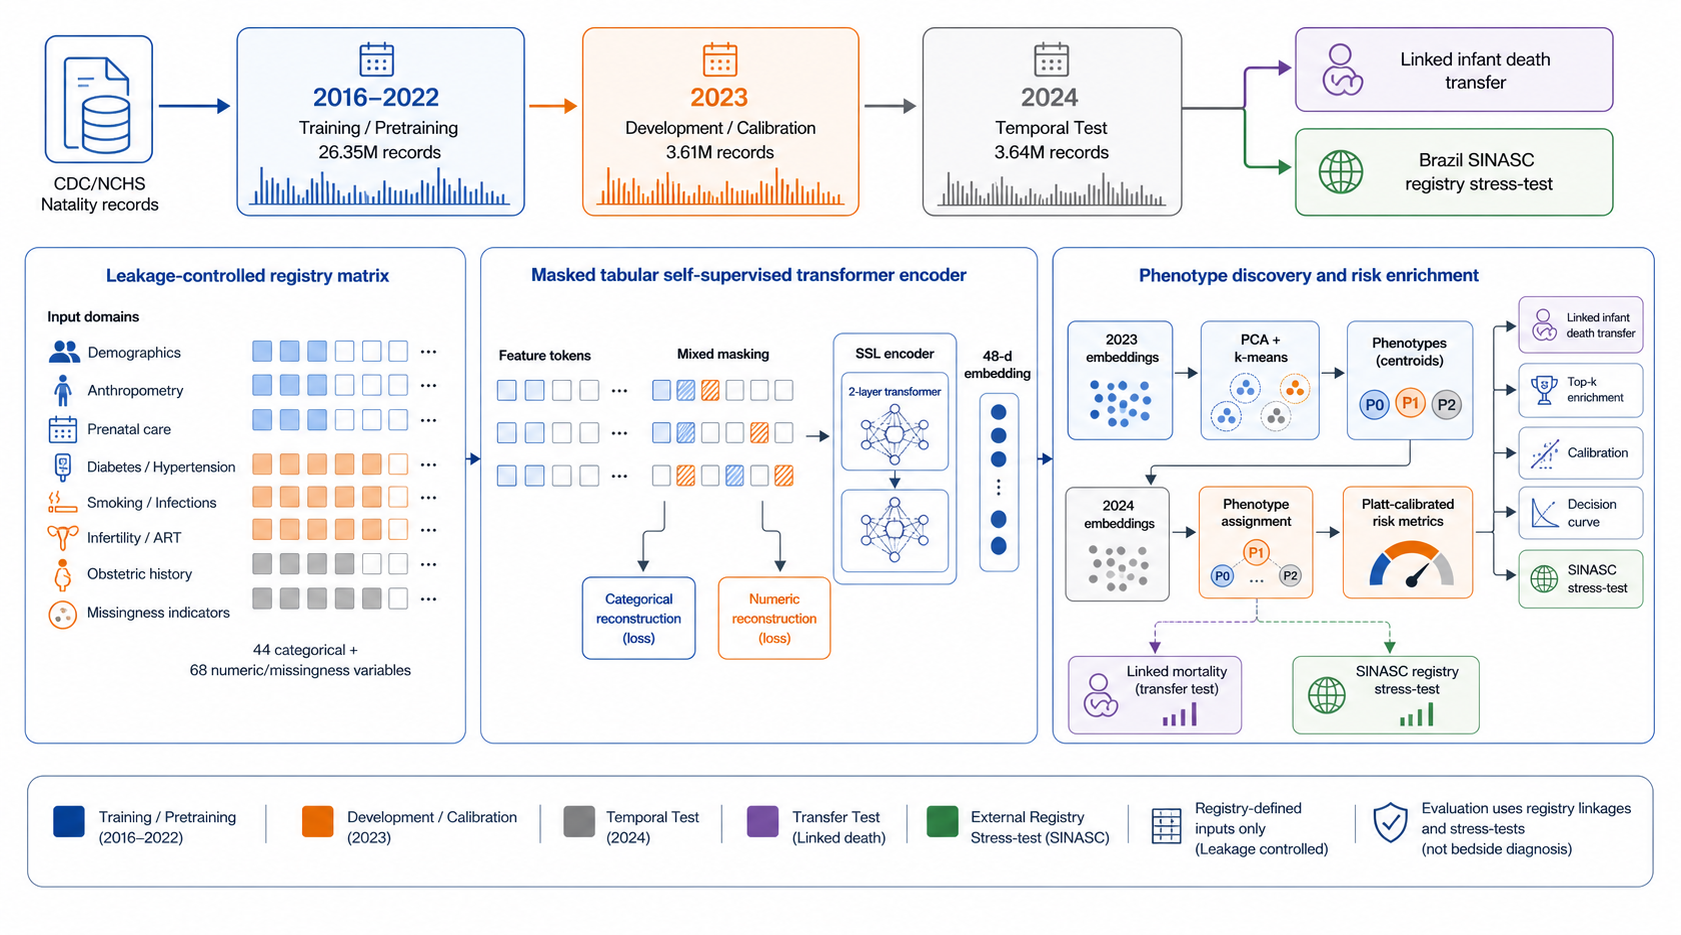
\includegraphics[width=\textwidth]{Figure_1_study_design_ssl_pipeline.png}
\caption{\textbf{Study design and masked tabular self-supervised phenotyping workflow.} The workflow begins with CDC/NCHS Natality public-use records and a calendar-time split: 2016--2022 records were used for supervised training and full-scale SSL pretraining, 2023 records for development and calibration, and 2024 records for temporal testing. Leakage-controlled U.S. Natality input groups included maternal demographics, anthropometry, prenatal care, diabetes and hypertensive disorders, smoking and infections, infertility and ART variables, obstetric history, and missingness indicators. Categorical and numeric/missingness variables were represented as feature tokens, randomly masked, and passed through a two-layer transformer encoder trained with masked categorical and numeric reconstruction losses to generate 48-dimensional record embeddings. Phenotype centroids were fit on 2023 SSL embeddings after PCA reduction and applied to 2024 embeddings using fixed centroids. Downstream models were Platt recalibrated and evaluated using AUPRC, top-risk enrichment, calibration, decision curves, and subgroup robustness. Fixed phenotype assignments were additionally evaluated in linked infant death records and in a separately trained SINASC registry stress-test. Labels from 2024 and transfer endpoints were used only for evaluation.}
\label{fig1}
\end{figure}

\subsection{Input variables}\label{subsec:inputs}

Inputs were restricted to leakage-controlled public-use variables representing maternal and pregnancy characteristics rather than downstream outcome components. We treated a variable as leakage-controlled if it was not itself a component of the maternal, neonatal, linked infant-death, or SINASC outcome definitions and if it represented maternal background, pregnancy history, prenatal care, risk-factor reporting, or pregnancy characteristics recorded on the birth certificate rather than the outcome component being predicted. Variables included maternal age, body mass index, weight gain, prenatal visits, plurality, pre-pregnancy diabetes, gestational diabetes, pre-pregnancy hypertension, gestational hypertension, eclampsia, previous preterm birth, infertility treatment, fertility-enhancing drug use, assisted reproductive technology, previous cesarean delivery, smoking, selected infections, and missingness indicators (Figure~\ref{fig1}). The SSL encoder used 112 feature tokens: 44 categorical fields, 12 continuous or ordered numeric fields, and 56 explicit missingness indicators. This count refers to input fields or indicators rather than one-hot-expanded dummy variables. Categorical missing values were represented as an explicit missing category, unseen categorical levels were mapped to an unknown category, and numeric values were standardized using training-period means and standard deviations with missing numeric values set to zero after standardization. Missingness indicators were retained because documentation patterns may carry predictive information in registry data; they were interpreted cautiously because missingness can also reflect access to care, coding practices, and institutional reporting rather than biological risk.

\subsection{Outcomes}\label{subsec:outcomes}

The primary maternal endpoint was core maternal morbidity, defined as maternal transfusion, ruptured uterus, unplanned hysterectomy, or maternal intensive care unit admission. These variables correspond to birth-certificate maternal morbidity fields used in national vital statistics reporting, but they are narrower than fully adjudicated severe maternal morbidity definitions \cite{nchs_natality_2024_userguide,luke2018smm}. The primary neonatal endpoint was a severe neonatal composite that excluded neonatal intensive care unit admission and was defined using very low birthweight below 1500 g, 5-minute Apgar score below 7, ventilation for more than 6 hours, or newborn seizures. Neonatal intensive care unit admission was excluded from the primary neonatal composite to reduce sensitivity to institutional practice patterns. These outcomes should be interpreted as registry-defined endpoints, not as clinically adjudicated electronic health record outcomes. The neonatal composite deliberately combined clinically serious but heterogeneous events and includes very low birthweight, which is closely related to prematurity and well-known obstetric risk factors; therefore, enrichment was interpreted as a severe-risk signal rather than as evidence for one specific neonatal pathophysiology.

\subsection{Linked birth/infant death transfer endpoint}\label{subsec:linked-infant-death}

To test whether fixed SSL phenotypes were associated with a more severe endpoint not used in SSL pretraining or phenotype discovery, we parsed the CDC/NCHS 2024 period/2023 cohort linked birth/infant death public-use file \cite{nchs_linked_2024_userguide}. Following the NCHS cohort-file construction guidance, 2023 denominator births were linked to 2023 and 2024 numerator infant death records using the cohort sequence number and year-of-death fields. The linked cohort contained 3,596,017 births and 19,743 infant deaths. We exported SSL embeddings for the linked cohort using the fixed full-scale encoder and assigned phenotypes using the fixed 2023 Natality development centroids. Infant death labels were not used to train the SSL encoder or to fit phenotype centroids. We evaluated infant death, neonatal death before 28 days, early neonatal death before 7 days, and postneonatal death from 28 days to one year.

For the linked severe-endpoint transfer analysis, we also fit descriptive logistic regression models with phenotype 2 as the reference group. The maternal-registry adjusted model included maternal age, body mass index, prenatal visits, gestational weight gain, diabetes, hypertensive disorders, previous preterm birth, infertility treatment, fertility drug use, assisted reproductive technology, previous cesarean delivery, smoking, selected infections, plurality, and infant sex. A second attenuation model additionally adjusted for gestational age and birthweight extracted from the linked denominator file. Because gestational age and birthweight lie close to the infant-death pathway, this second model was interpreted descriptively rather than as a deployable pre-delivery prediction model.

To benchmark the linked phenotype transfer against a supervised alternative, we trained an all-input LightGBM model for the primary severe neonatal endpoint using the same 3,500,000-record 2016--2022 training sample as the main supervised comparison, fit Platt recalibration in all 2023 development records, and transferred the calibrated severe-neonatal score to the linked birth/infant death cohort. Infant death labels were not used to train or recalibrate this supervised score. We compared infant-death enrichment among births selected by the predefined high-risk phenotype 0 with births selected by the supervised score at the same 4.58\% cohort fraction and at additional top-risk fractions.

\subsection{Independent SINASC public-registry stress-test}\label{subsec:sinasc}

To test whether the analytic workflow could be rebuilt outside the CDC/NCHS ecosystem, we downloaded Brazil OpenDataSUS/SINASC 2023 and 2024 public-use birth registry CSV files and the official SINASC structure dictionary \cite{opendatasus_sinasc,sinasc_structure_dictionary}. The 2023 file contained 2,537,576 records and the 2024 file contained 2,389,325 records. We profiled all 62 SINASC fields, extracted dictionary context for 60 fields, and mapped the available variables to the nearest Natality-compatible concept families. Leakage-controlled predictor domains included maternal age, race/color, marital status, education, residential geography, prior live births, prior fetal losses, prior cesarean delivery, prenatal care timing and visit count, plurality, and infant sex. Gestational age, birthweight, 5-minute Apgar score, and congenital anomaly were used only to construct SINASC birth-status endpoints and were not included in the predictor matrix or SSL pretraining inputs. Several U.S. Natality feature families had no direct SINASC public-use analogue, including maternal body mass index and weight gain, smoking, diabetes, hypertensive disorders, selected infections, infertility and assisted reproductive technology, WIC/payment variables, current maternal morbidity fields, neonatal intensive care unit admission, ventilation, and seizures.

Because of this feature non-overlap, the SINASC analysis was defined as a workflow-level registry stress-test rather than fixed U.S.-encoder validation. We built a separate harmonized SINASC matrix with 46 leakage-controlled predictor variables including missingness indicators, trained a separate masked tabular SSL encoder on 500,000 sampled 2023 records, used a disjoint 200,000-record 2023 development sample for phenotype selection and calibration, and evaluated the full 2024 SINASC year once. Severe SINASC birth-status outcome combined very preterm birth before 32 weeks, very low birthweight below 1500 g, 5-minute Apgar score below 7, or congenital anomaly. Broad birth-status outcome combined preterm birth before 37 weeks, low birthweight below 2500 g, 5-minute Apgar score below 7, or congenital anomaly. The stress-test compared overlap-input LightGBM, SSL embedding logistic regression, SSL plus phenotype logistic regression, and phenotype-only logistic regression.

\subsection{Masked tabular SSL encoder}\label{subsec:ssl}

The SSL encoder represented categorical inputs as learned feature tokens and projected numeric variables into the same token space, following the general logic of tabular representation learning and transformer-based tabular models \cite{yoon2020vime,huang2020tabtransformer,somepalli2021saint,gorishniy2021revisiting}. Feature-position embeddings identified each variable. During pretraining, categorical and numeric tokens were randomly masked. A development-only reconstruction ablation supported a mask rate of 0.35 with model dimension 48 and two transformer layers. The final encoder used four attention heads and was trained to reconstruct masked categorical variables using cross-entropy loss and masked numeric variables using mean squared error. Record-level embeddings were generated by mean pooling encoded feature tokens rather than a classification token because the objective was input reconstruction and downstream phenotype discovery rather than direct supervised classification (Figure~\ref{fig1}).

The final encoder was pretrained on all 26,345,765 records from 2016--2022 using a row-group streaming pipeline and CUDA PyTorch. The final 2023 development reconstruction loss was 0.1859, with categorical loss 0.3013 and numeric loss 0.1112. After training, the encoder was held fixed and used to export 48-dimensional embeddings for all 3,605,081 2023 development records, all 3,638,436 records in the 2024 temporal test year, and a 3,500,000-record 2016--2022 training sample for incremental supervised comparisons.

\subsection{Phenotype discovery}\label{subsec:phenotype-discovery}

Phenotype discovery was performed on all 2023 SSL embeddings only (Figure~\ref{fig1}). Embeddings were standardized and reduced with PCA. Candidate k-means solutions from $k = 3$ to $k = 8$ were evaluated using silhouette score, Davies-Bouldin index, Calinski-Harabasz index, and minimum cluster proportion. The selected solution used $k = 3$ and 16 PCA components, explaining 97.22\% of embedding variance in the full-scale downstream analysis. Phenotype labels were ordered by 2023 severe neonatal outcome rate so that phenotype 0 denoted the highest-risk group. The 2023 centroids were fixed and then applied to 2024 embeddings. Labels from 2024 were not used for clustering or cluster selection.

\subsection{Supervised baselines and incremental comparison}\label{subsec:baselines}

We trained LightGBM supervised baselines using sampled 2016--2022 training data (500,000 records per year; 3,500,000 records total) \cite{ke2017lightgbm}. The training sample was used for computational tractability while retaining calendar-time separation and full-year development and test evaluation. Two supervised feature sets were evaluated during development: a comorbidity-focused subset and all leakage-controlled inputs. The main full-year incremental experiment tested three feature sets on all 3,638,436 temporal test records from 2024: all leakage-controlled inputs, SSL embeddings alone, and all leakage-controlled inputs plus SSL embeddings. This comparison held the gradient-boosted tree model family constant when comparing original registry inputs with SSL embeddings. Downstream logistic models were interpreted separately as simple calibrated models on SSL-derived representations and were not used to claim model-family equivalence with all-input LightGBM. These models used the 3,500,000-record training sample, all 3,605,081 development records for Platt recalibration, and all 3,638,436 temporal test records from 2024 for final evaluation.

\subsection{Downstream SSL risk models and calibration}\label{subsec:calibration}

Downstream logistic models evaluated three SSL-derived feature sets: SSL embeddings alone, phenotype labels alone, and SSL embeddings plus phenotype labels. Logistic models used standardized inputs, the lbfgs solver, balanced class weights, and default L2 regularization. Within 2023 development data, a stratified 60\%/40\% split separated model fitting from Platt recalibration \cite{platt1999probabilistic}. Platt models were fit only in development data, and 2024 labels were reserved for final evaluation. Test metrics were then computed once on the full 2024 temporal test year. Performance metrics included AUROC, AUPRC, AUPRC divided by outcome prevalence, top 1\% risk enrichment, Brier score, and 10-bin expected calibration error. AUPRC and top-risk enrichment were emphasized because the endpoints were imbalanced and clinically relevant use would be closer to risk enrichment than definitive diagnosis \cite{davis2006precision}. Bootstrap confidence intervals were computed for full-year LightGBM and SSL-derived model metrics using 200 bootstrap iterations.

\subsection{Clinical utility, subgroup robustness, and model interpretation}\label{subsec:utility-interpretability}

To make the clinical-decision relevance explicit, we summarized observed event rates, recall, enrichment over prevalence, and number needed to evaluate among the highest-risk 0.5\%, 1\%, 2\%, and 5\% of 2024 test records. Number needed to evaluate was defined descriptively as the inverse of the observed event rate in the selected top-risk stratum. We also performed decision-curve analysis across risk thresholds of 0.25\% to 5\% for maternal core morbidity and 2\% to 20\% for severe neonatal outcome, comparing model-guided selection against treat-all and treat-none reference strategies \cite{vickers2006decision}. These threshold grids were chosen to cover low-prevalence enrichment scenarios rather than to define clinical action thresholds. The analyses were framed as retrospective triage or chart-review scenarios; no clinical action threshold was proposed because valid thresholds would require explicit intervention options, harms, resource constraints, local prevalence, and prospective workflow evaluation. Subgroup robustness was assessed for maternal age, body mass index, diabetes, hypertensive disorders, infertility or assisted reproductive technology, plurality, and prior cesarean delivery. These subgroup analyses were treated as screening checks for heterogeneity rather than a complete fairness audit. For phenotype interpretation, we summarized gestational age, birthweight, preterm birth, low birthweight, very low birthweight, and low 5-minute Apgar rate by assigned phenotype in the full 2024 test year. In the linked birth/infant death cohort, we also grouped ICD-10 underlying causes of infant death into clinically interpretable categories and estimated cause-specific enrichment in the predefined high-risk phenotype.

\subsection{Stability and sensitivity analyses}\label{subsec:stability}

Phenotype stability was assessed using repeated 80\% resampling of 2023 development embeddings with a 500,000-record cap per resample for computational tractability. Resampled cluster labels were compared with primary labels using adjusted Rand index and normalized mutual information. Dimensionality sensitivity was assessed by fitting PCA on all 2023 SSL embeddings and evaluating downstream models using 5, 10, 20, or 32 principal components, then applying the fixed PCA transform to 2024. These analyses were designed to test whether the phenotype structure and risk-enrichment signal were robust to resampling and compression of the SSL representation.

\subsection{Software and reproducibility}\label{subsec:software}

Data parsing and modeling were implemented in Python. Key packages included pandas, pyarrow, scikit-learn, LightGBM, PyTorch, NumPy, and matplotlib. The main random seed was 20260525. Source scripts, generated source-data tables, and figure-building scripts are provided with the submission as Additional file 1 and use the official public-use sources described below.

\section{Results}\label{sec:results}

\subsection{Calendar-time cohort and analytic endpoints}\label{subsec:calendar-results}

The full temporal analytic dataset included 26,345,765 records from 2016--2022, 3,605,081 records from 2023, and 3,638,436 records from 2024. The calendar-time split separated training and SSL pretraining from development, calibration, and final-year testing (Figure~\ref{fig1}). In the full 2024 temporal test year, maternal core morbidity occurred in 28,042 of 3,638,436 records (0.771\%) and the severe neonatal composite excluding neonatal intensive care unit admission occurred in 169,135 of 3,638,436 records (4.649\%). The primary endpoints were therefore imbalanced, particularly maternal core morbidity, supporting the use of AUPRC and top-risk enrichment in addition to AUROC.

Figure~\ref{fig1} summarizes the analysis design. Input variables were grouped into maternal demographic, anthropometric, prenatal-care, cardiometabolic, infection, infertility-treatment, obstetric-history, and missingness domains. The SSL encoder learned 48-dimensional record embeddings through masked categorical and numeric reconstruction. Phenotype discovery and risk evaluation were performed downstream using 2023 embeddings for phenotype fitting and 2024 embeddings for final evaluation.

\begin{table}[!htbp]
\caption{\textbf{Calendar-time analytic split and primary endpoint prevalence.}}
\label{tab:cohort-endpoints}
\centering
\scriptsize
\setlength{\tabcolsep}{3pt}
\begin{tabular*}{\textwidth}{@{\extracolsep{\fill}}lllll@{}}
\toprule
Period & Role & Records & Maternal morbidity & Severe neonatal \\
\midrule
2016--2022 & Training / pretraining & 26,345,765 & 158,866 (0.603\%) & 1,060,190 (4.024\%) \\
2023 & Development / calibration & 3,605,081 & 27,365 (0.759\%) & 163,961 (4.548\%) \\
2024 & Temporal test & 3,638,436 & 28,042 (0.771\%) & 169,135 (4.649\%) \\
\bottomrule
\end{tabular*}
\end{table}

\subsection{Full-year supervised and SSL-derived risk-enrichment comparison}\label{subsec:risk-comparison}

In the full 3,638,436-record 2024 temporal test year, all-input LightGBM remained the strongest pure predictor for both primary endpoints (Figure~\ref{fig2}). For maternal core morbidity, all-input LightGBM achieved AUROC 0.6905, AUPRC 0.0234, and top 1\% enrichment 7.04-fold. SSL embeddings alone in LightGBM achieved AUROC 0.6584, AUPRC 0.0170, and top 1\% enrichment 4.77-fold. Adding SSL embeddings to all leakage-controlled inputs did not improve performance, with AUROC 0.6901, AUPRC 0.0230, and top 1\% enrichment 6.99-fold.

For severe neonatal outcome, all-input LightGBM achieved AUROC 0.7613, AUPRC 0.3009, and top 1\% enrichment 15.20-fold. SSL embeddings alone in LightGBM achieved AUROC 0.7145, AUPRC 0.2184, and top 1\% enrichment 11.58-fold. All inputs plus SSL embeddings achieved AUROC 0.7612, AUPRC 0.3008, and top 1\% enrichment 15.16-fold. These full-year supervised results established a strong prediction benchmark and confirmed that the SSL-derived models should not be framed as superior prediction models.

SSL embeddings nevertheless retained risk-enrichment structure above baseline prevalence. In downstream SSL-derived logistic models, SSL plus phenotype achieved severe neonatal AUPRC 0.1859 and maternal core morbidity AUPRC 0.0167. Phenotype labels alone were weaker predictors, but they provided a compact representation for clinical profiling. The incremental experiment is important for interpretation: the SSL representation carried outcome-relevant structure, but it did not replace or consistently improve a strong supervised model using the original registry variables.

\begin{table}[!htbp]
\caption{\textbf{Full-year 2024 temporal-test performance of all-input and SSL feature sets in LightGBM.}}
\label{tab:model-performance}
\centering
\scriptsize
\setlength{\tabcolsep}{3pt}
\begin{tabular*}{\textwidth}{@{\extracolsep{\fill}}lcccccc@{}}
\toprule
Feature set & \multicolumn{3}{c}{Maternal core morbidity} & \multicolumn{3}{c}{Severe neonatal composite} \\
\cmidrule(lr){2-4}\cmidrule(lr){5-7}
 & AUROC & AUPRC & Top 1\% enrich. & AUROC & AUPRC & Top 1\% enrich. \\
\midrule
All inputs & 0.691 & 0.0234 & 7.04$\times$ & 0.761 & 0.3009 & 15.20$\times$ \\
SSL embeddings & 0.658 & 0.0170 & 4.77$\times$ & 0.715 & 0.2184 & 11.58$\times$ \\
All inputs + SSL & 0.690 & 0.0230 & 6.99$\times$ & 0.761 & 0.3008 & 15.16$\times$ \\
\bottomrule
\end{tabular*}
\end{table}

\begin{figure}[!htbp]
\centering
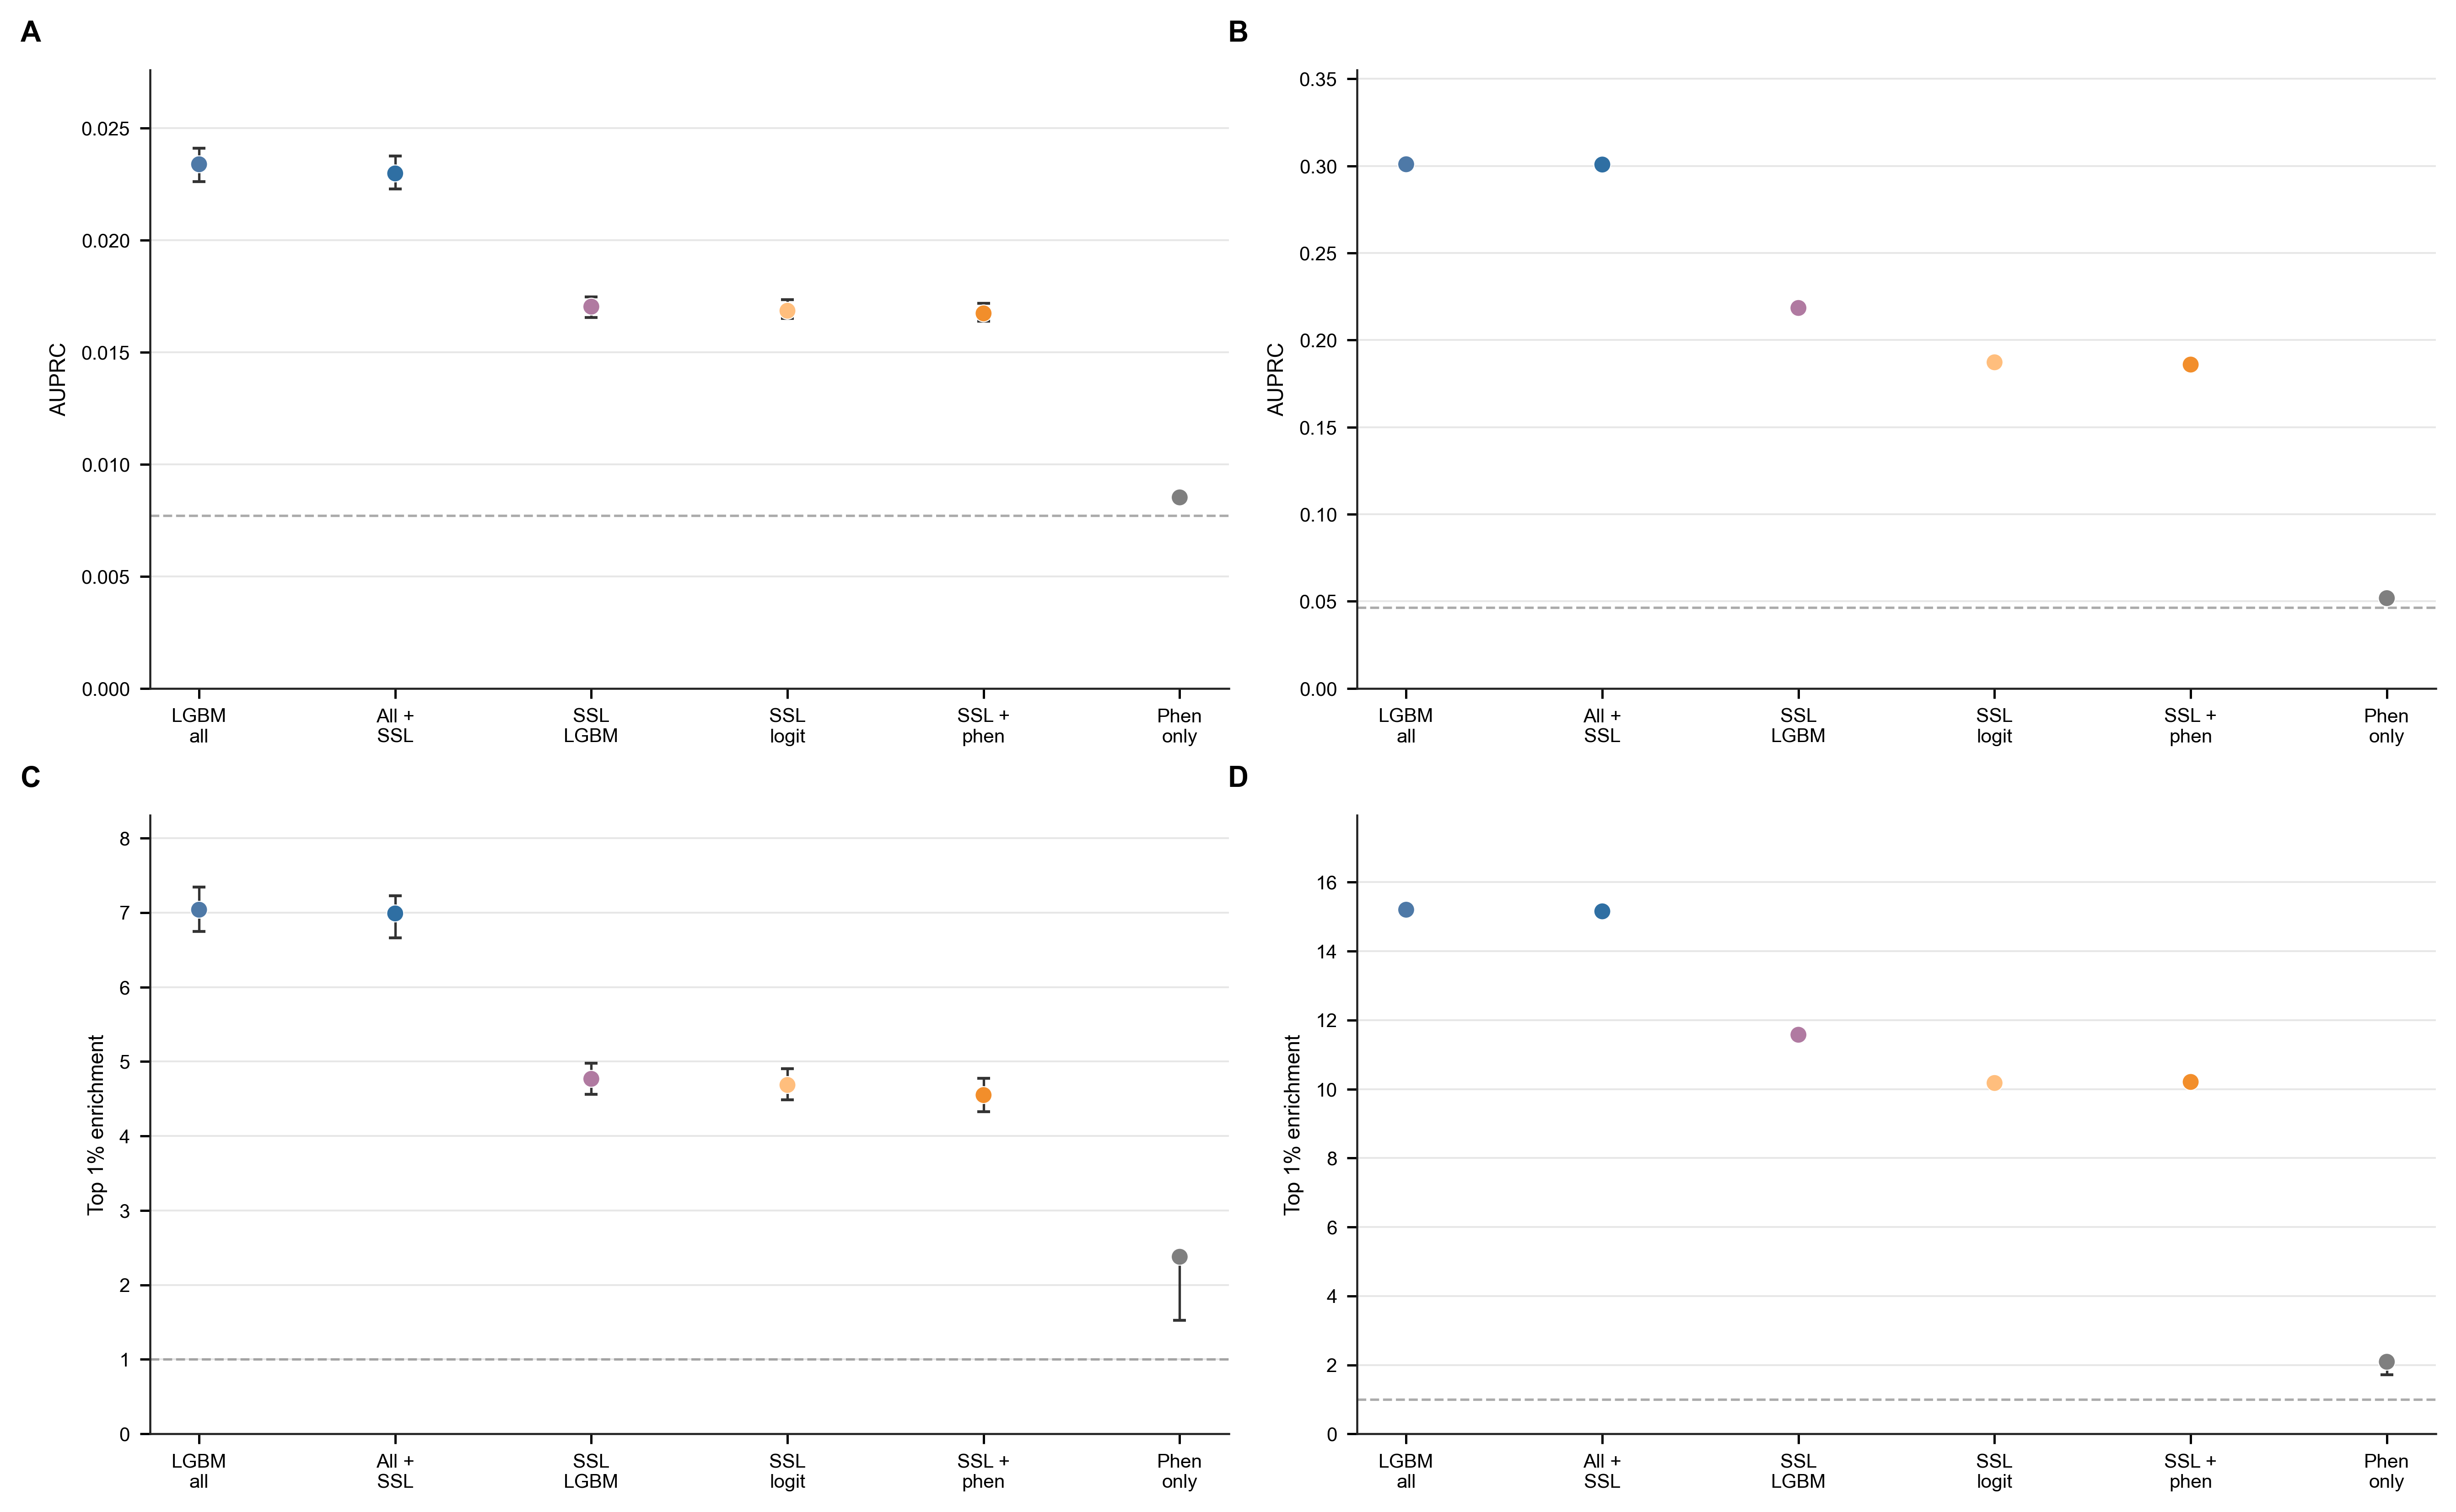
\includegraphics[width=\textwidth]{Figure_2_full_year_model_summary.png}
\caption{\textbf{Full-year 2024 comparison of supervised and SSL-derived risk-enrichment models.} Models were developed and recalibrated using all 3,605,081 development records from 2023 and evaluated on all 3,638,436 temporal test records from 2024. \textbf{A,} AUPRC for maternal core morbidity. \textbf{B,} AUPRC for severe neonatal outcome. \textbf{C,} Top 1\% risk enrichment for maternal core morbidity. \textbf{D,} Top 1\% risk enrichment for severe neonatal outcome. Supervised incremental LightGBM models tested all leakage-controlled inputs, SSL embeddings alone, and all leakage-controlled inputs plus SSL embeddings. SSL-derived logistic models used SSL embeddings alone, phenotype labels alone, or SSL embeddings plus phenotype labels. Error bars show bootstrap 95\% confidence intervals where available. Dashed horizontal lines indicate endpoint prevalence for AUPRC panels and no enrichment for top-risk panels.}
\label{fig2}
\end{figure}

\subsection{SSL phenotype discovery and outcome enrichment}\label{subsec:phenotype-results}

The full 2023 SSL embeddings supported a three-phenotype solution (Figure~\ref{fig3}A--C). When fixed 2023 centroids were applied to the full 2024 test year, phenotype 0 contained 172,524 records, phenotype 1 contained 1,677,612 records, and phenotype 2 contained 1,788,300 records. Cluster selection favored $k = 3$ because it provided the strongest silhouette score and a reproducible smaller high-risk phenotype among candidate solutions.

The phenotype solution was stable across repeated capped 80\% resampling of 2023 development embeddings (Figure~\ref{fig3}D). Median adjusted Rand index was 0.997 and median normalized mutual information was 0.991 versus the primary labels. The median minimum cluster proportion was 0.046, indicating that the smaller phenotype was reproducibly recovered rather than appearing as an isolated random fragment.

Phenotype 0 was enriched for both adverse outcomes in the full 2024 test year (Figure~\ref{fig3}E). Maternal core morbidity was 1.271\% in phenotype 0, compared with 0.815\% in phenotype 1 and 0.681\% in phenotype 2. Severe neonatal outcome was 8.249\% in phenotype 0, compared with 4.815\% in phenotype 1 and 4.145\% in phenotype 2. Bootstrap confidence intervals supported this enrichment pattern. Prototype profiling showed that the high-risk phenotype differed from the other phenotypes across selected maternal and pregnancy characteristics, including BMI, prenatal visits, prior preterm birth, prior cesarean delivery, smoking, and missingness patterns (Figure~\ref{fig3}F). These phenotypes should be interpreted as latent representation groups associated with risk enrichment, not causal clinical subtypes.

\begin{figure}[!htbp]
\centering
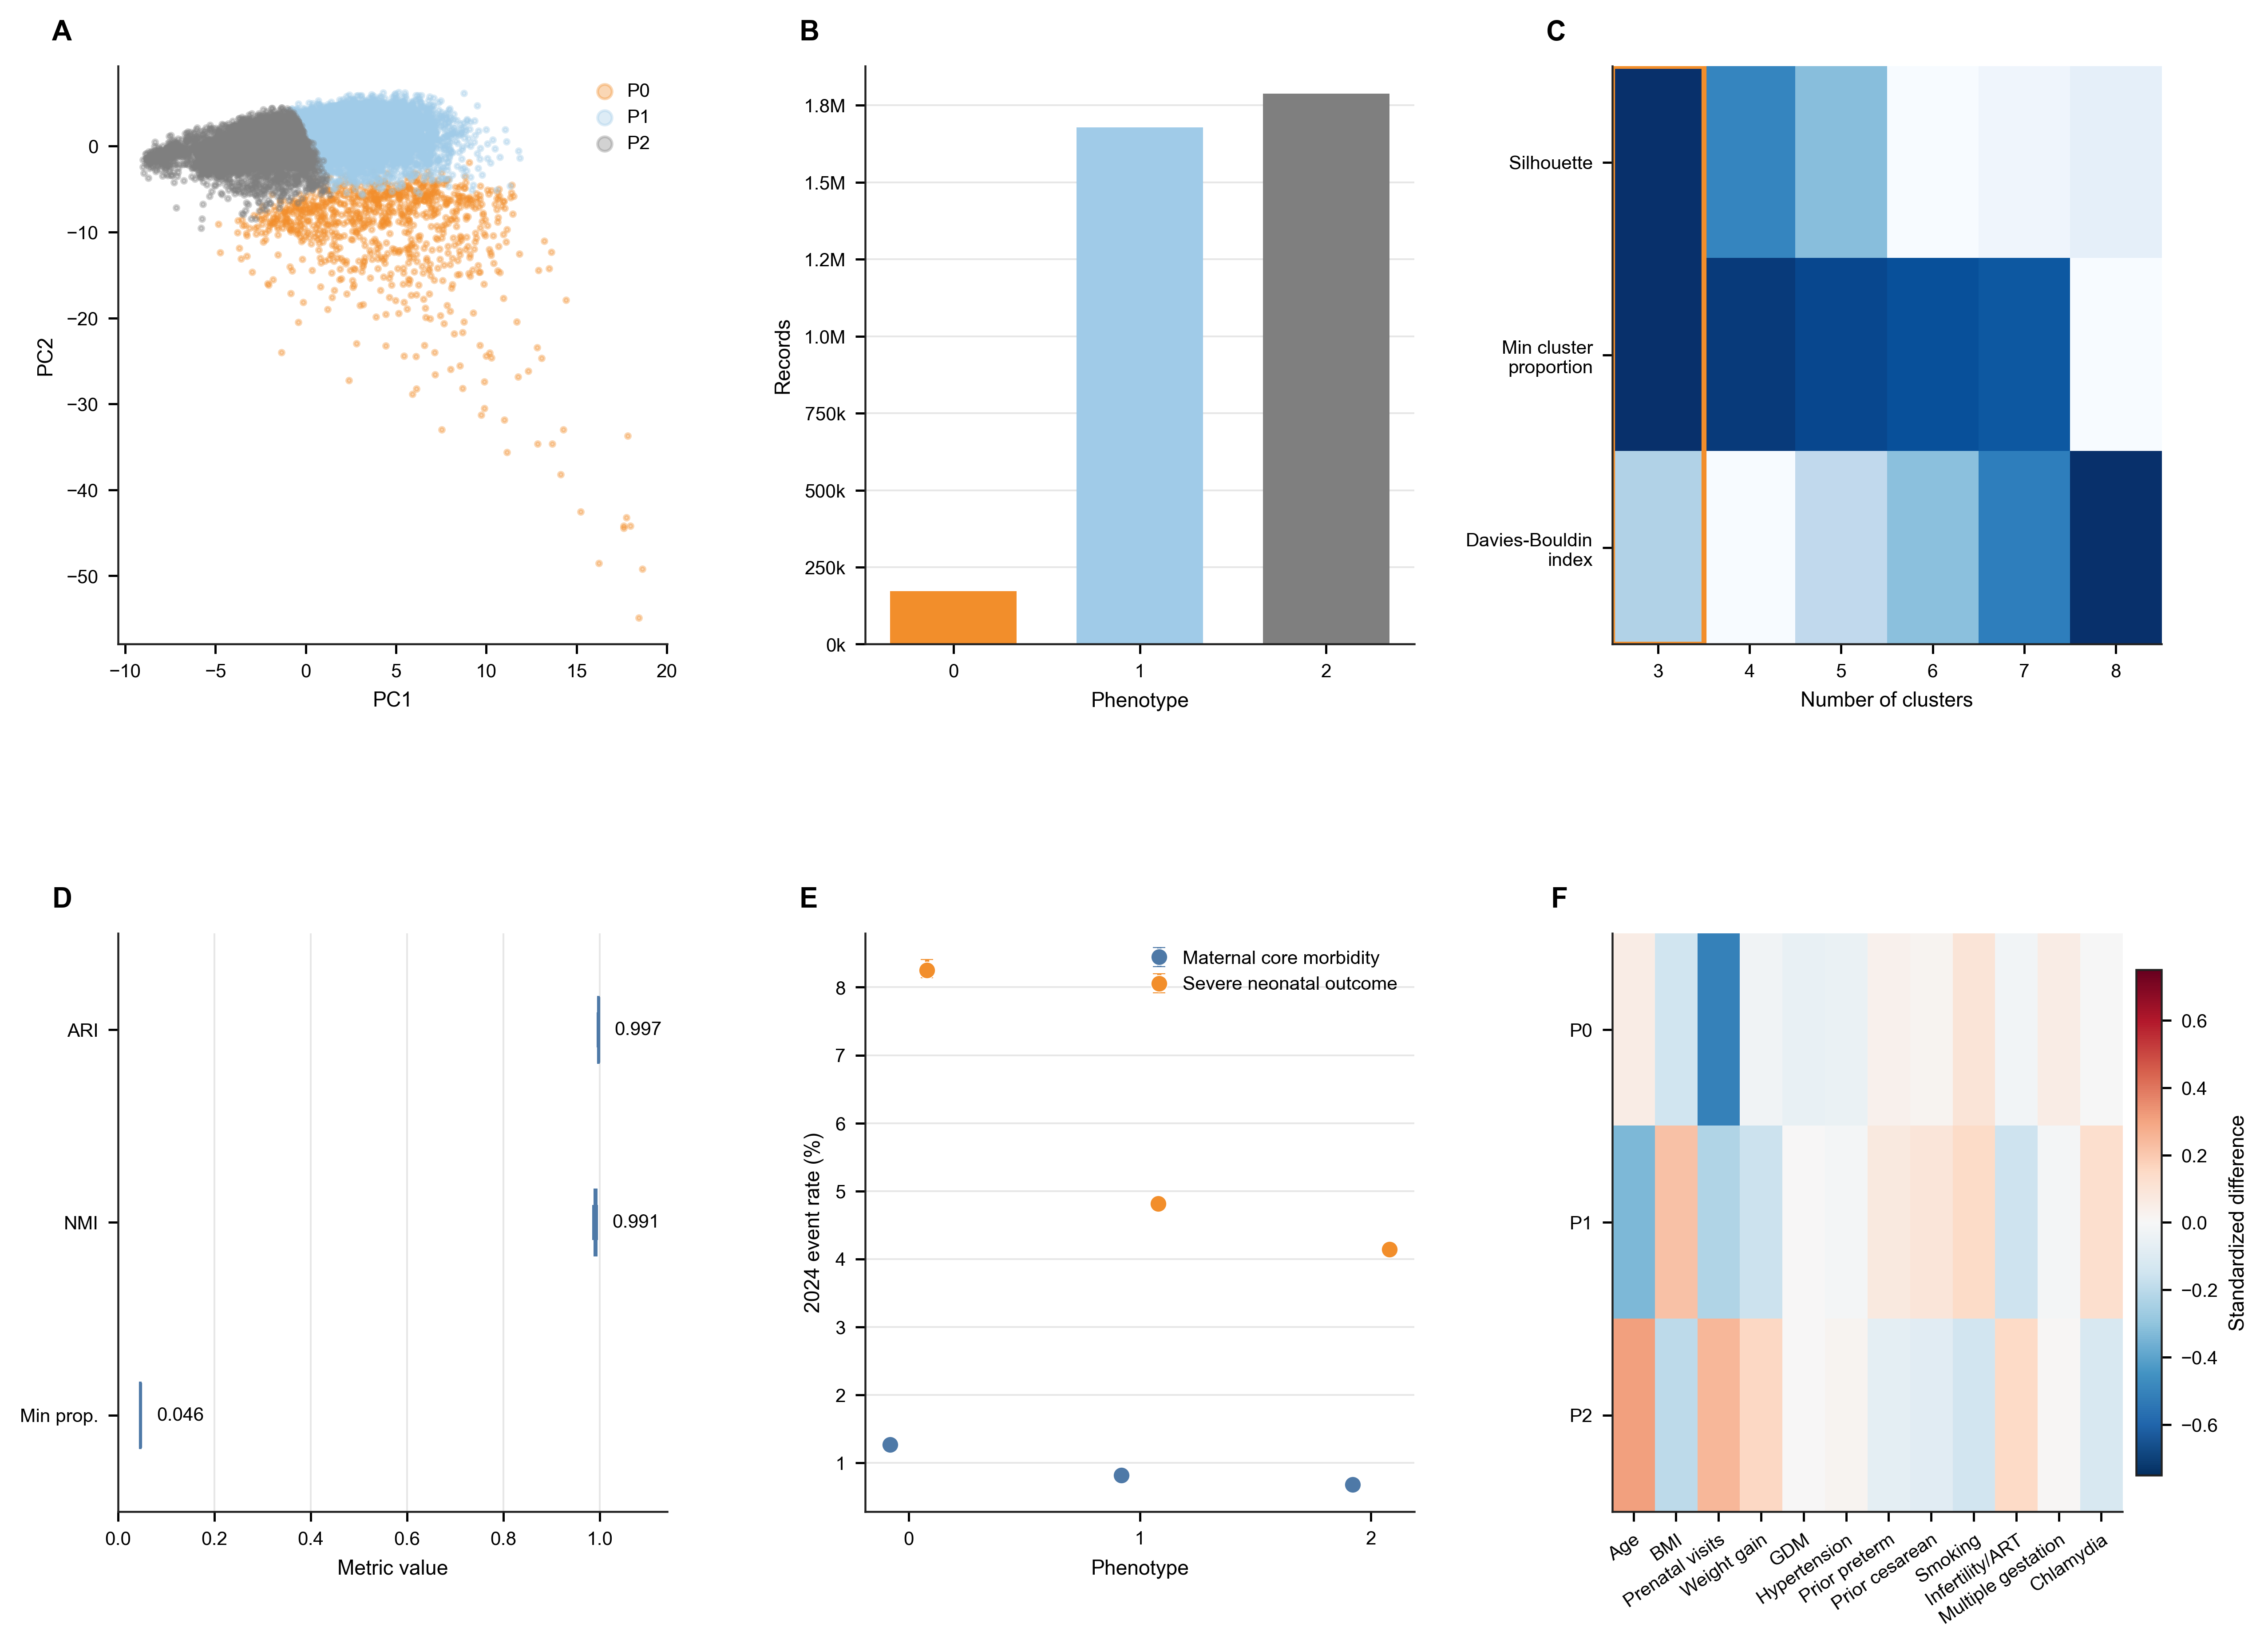
\includegraphics[width=\textwidth]{Figure_3_ssl_phenotype_discovery.png}
\caption{\textbf{SSL phenotype discovery, stability, and clinical enrichment.} \textbf{A,} PCA visualization of full 2023 SSL embeddings colored by the three selected phenotype labels. \textbf{B,} Phenotype sizes after applying fixed 2023 centroids to 2024 SSL embeddings. \textbf{C,} Development-only cluster-selection diagnostics across candidate $k$ values. Higher color intensity indicates a more favorable value after within-metric scaling; the Davies--Bouldin index is inverted so lower raw values are favored. \textbf{D,} Development-set phenotype stability across repeated capped 80\% 2023 resampling, summarized by median and interquartile range for adjusted Rand index, normalized mutual information, and minimum cluster proportion. \textbf{E,} Maternal and neonatal outcome rates in 2024 by assigned phenotype, with bootstrap 95\% confidence intervals. \textbf{F,} Standardized profile of selected maternal and pregnancy characteristics across assigned 2024 phenotypes. Phenotype labels represent latent SSL-derived groups associated with outcome enrichment; they should not be interpreted as causal clinical subtypes.}
\label{fig3}
\end{figure}

\subsection{Calibration and dimensionality sensitivity}\label{subsec:calibration-results}

Platt recalibration mapped SSL downstream scores to a more interpretable probability scale (Figure~\ref{fig4}A--D), while preserving the distinction between calibrated retrospective risk estimates and deployable clinical probabilities. Platt parameters were fit in 2023 development data and then applied unchanged to the 2024 temporal test year. For severe neonatal outcome, SSL plus phenotype achieved AUPRC 0.1859 with bootstrap 95\% confidence interval 0.1840 to 0.1879. Top 1\% enrichment was 10.21-fold with bootstrap 95\% confidence interval 10.10 to 10.34. Its Brier score was 0.0413 (95\% CI, 0.0412--0.0415) and expected calibration error was 0.0021 (95\% CI, 0.0019--0.0023). Maternal core morbidity showed lower absolute discrimination, consistent with lower event frequency, but SSL plus phenotype retained AUPRC 0.0167 (95\% CI, 0.0164--0.0172) and top 1\% enrichment of 4.55-fold (95\% CI, 4.33--4.78). Its Brier score was 0.0076 (95\% CI, 0.0075--0.0077) and expected calibration error was 0.00016 (95\% CI, 0.00012--0.00027). Calibration plots for SSL plus phenotype models showed close agreement between mean predicted risk and observed event rates after Platt recalibration, although calibration does not imply deployment readiness.

PCA-compression sensitivity indicated that the SSL signal was distributed across latent dimensions (Figure~\ref{fig4}E--F). Five to ten principal components were insufficient, particularly for severe neonatal outcome. For severe neonatal outcome, AUPRC increased from 0.0812 using 5 principal components to 0.1430 using 32 components and 0.1842 using the full 48-dimensional embedding. Top 1\% enrichment increased from 2.74-fold with 5 components to 7.49-fold with 32 components and 9.94-fold with the full embedding. This pattern suggests that the SSL representation was not reducible to a single dominant low-dimensional axis.

\begin{figure}[!htbp]
\centering
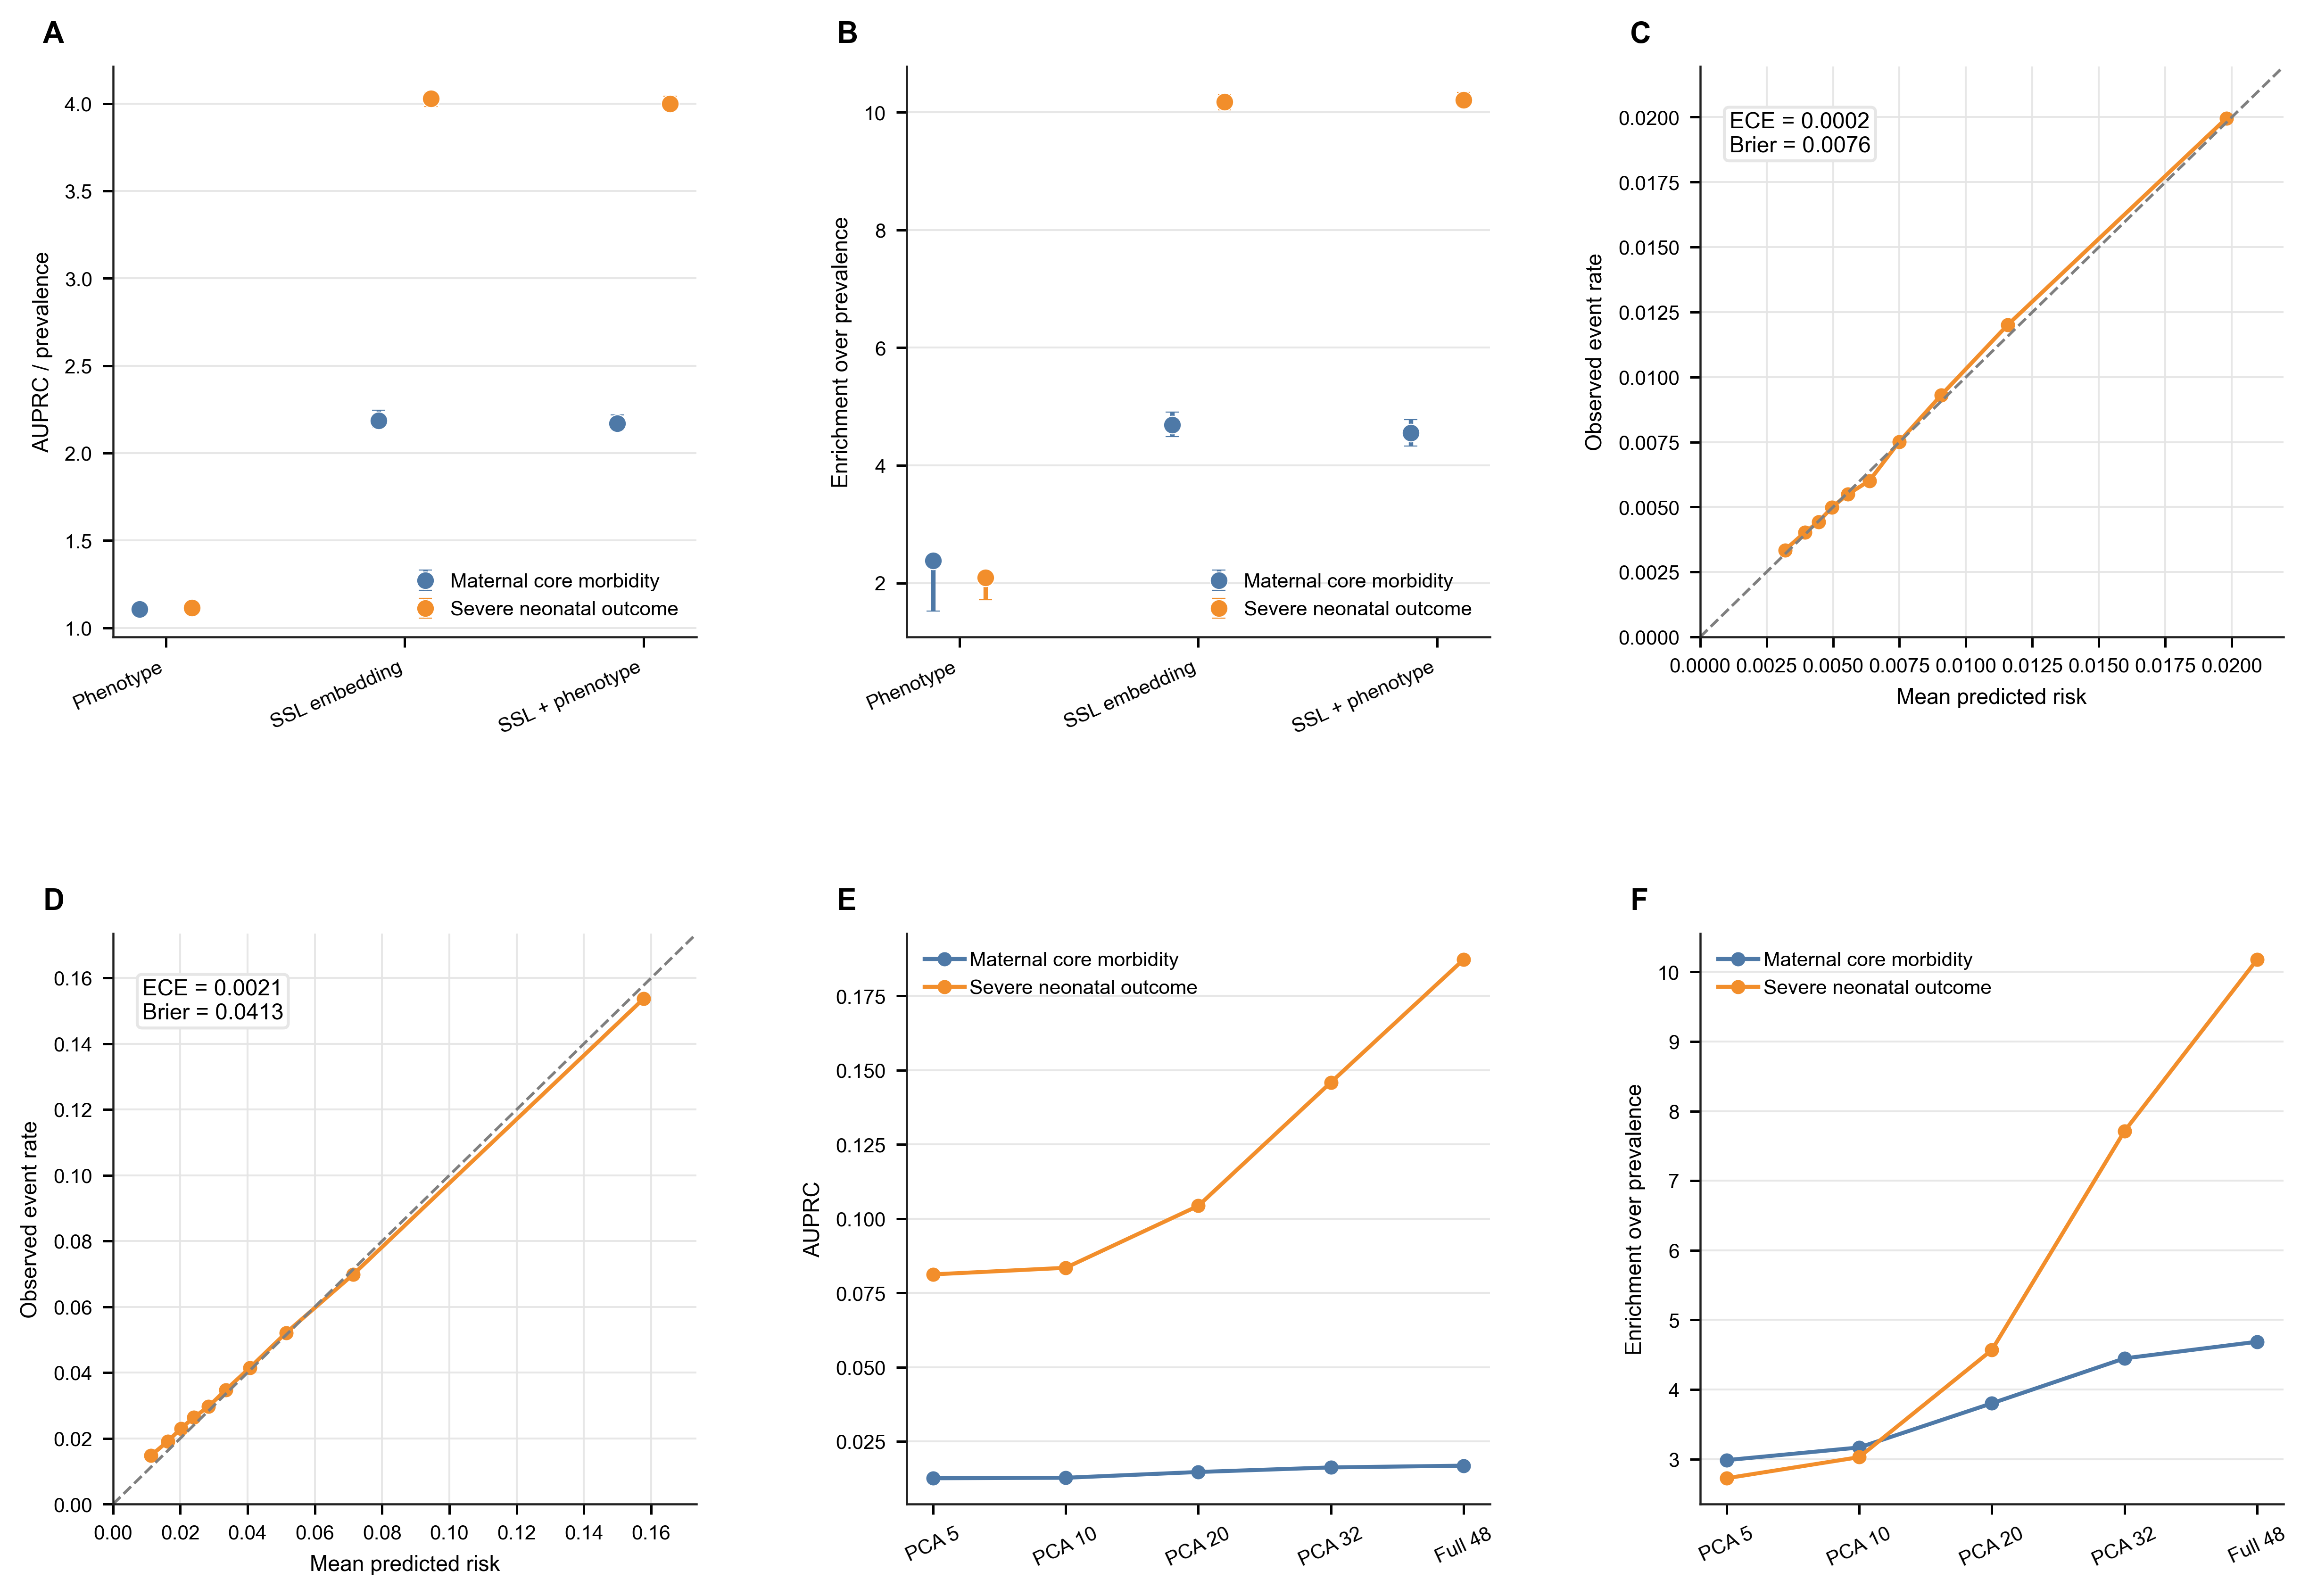
\includegraphics[width=\textwidth]{Figure_4_calibration_sensitivity.png}
\caption{\textbf{Calibration, risk-enrichment uncertainty, and SSL dimensionality sensitivity.} \textbf{A,} Bootstrap 95\% confidence intervals for Platt-calibrated AUPRC relative to endpoint prevalence across SSL-derived feature sets. \textbf{B,} Bootstrap 95\% confidence intervals for top 1\% enrichment across SSL-derived feature sets. \textbf{C,} Calibration plot for the SSL plus phenotype maternal core morbidity model, annotated with Platt-calibrated expected calibration error and Brier score. \textbf{D,} Calibration plot for the SSL plus phenotype severe neonatal outcome model, annotated with Platt-calibrated expected calibration error and Brier score. Dashed lines indicate ideal calibration. \textbf{E,} PCA-compression sensitivity for AUPRC after fitting PCA on 2023 SSL embeddings and applying the fixed transform to 2024. \textbf{F,} PCA-compression sensitivity for top 1\% enrichment. Five to ten principal components were insufficient, particularly for severe neonatal outcome, whereas 32 components retained most of the full 48-dimensional embedding signal. These results support a distributed SSL latent representation rather than a single dominant low-dimensional phenotype axis.}
\label{fig4}
\end{figure}

\subsection{Clinical utility and phenotype interpretation}\label{subsec:utility-results}

Top-risk summaries translated model scores into an enrichment scenario closer to screening or chart-review prioritization than binary diagnosis (Figure~\ref{fig5}A--B). For severe neonatal outcome, the overall prevalence in the full 2024 temporal test year was 4.649\%. Among the highest-risk 1\% of records by SSL plus phenotype score, the observed event rate was 47.45\%, corresponding to 10.21-fold enrichment over prevalence and a number needed to evaluate of 2.11. For maternal core morbidity, the overall prevalence was 0.771\%; the top 1\% event rate was 3.51\%, corresponding to 4.55-fold enrichment and a number needed to evaluate of 28.5. These results support risk enrichment but not standalone diagnostic use.

Decision-curve analysis showed positive but modest net benefit for SSL plus phenotype model-guided selection across the evaluated thresholds compared with treat-none and, across most thresholds, treat-all reference strategies (Figure~\ref{fig5}C--D). Phenotype-level birth-status profiles were consistent with expected clinical gradients: phenotype 0 had lower mean gestational age than phenotype 2 (37.90 versus 38.70 weeks), lower mean birthweight (3123 versus 3310 g), higher preterm birth rate (18.1\% versus 9.6\%), higher low-birthweight rate (13.5\% versus 6.6\%), higher very-low-birthweight rate (4.1\% versus 0.9\%), and higher low 5-minute Apgar rate (4.4\% versus 2.1\%). In linked infant death records, phenotype 0 was enriched most strongly for deaths assigned to perinatal conditions (5.36-fold over prevalence), with weaker but still elevated enrichment for congenital anomalies (2.30-fold), infection or respiratory causes (2.27-fold), other causes (2.12-fold), SIDS or ill-defined causes (1.78-fold), and external injury (1.63-fold). This pattern is consistent with a broad high-risk maternal and perinatal vulnerability phenotype, not a cause-specific diagnostic subtype.

\begin{figure}[!htbp]
\centering
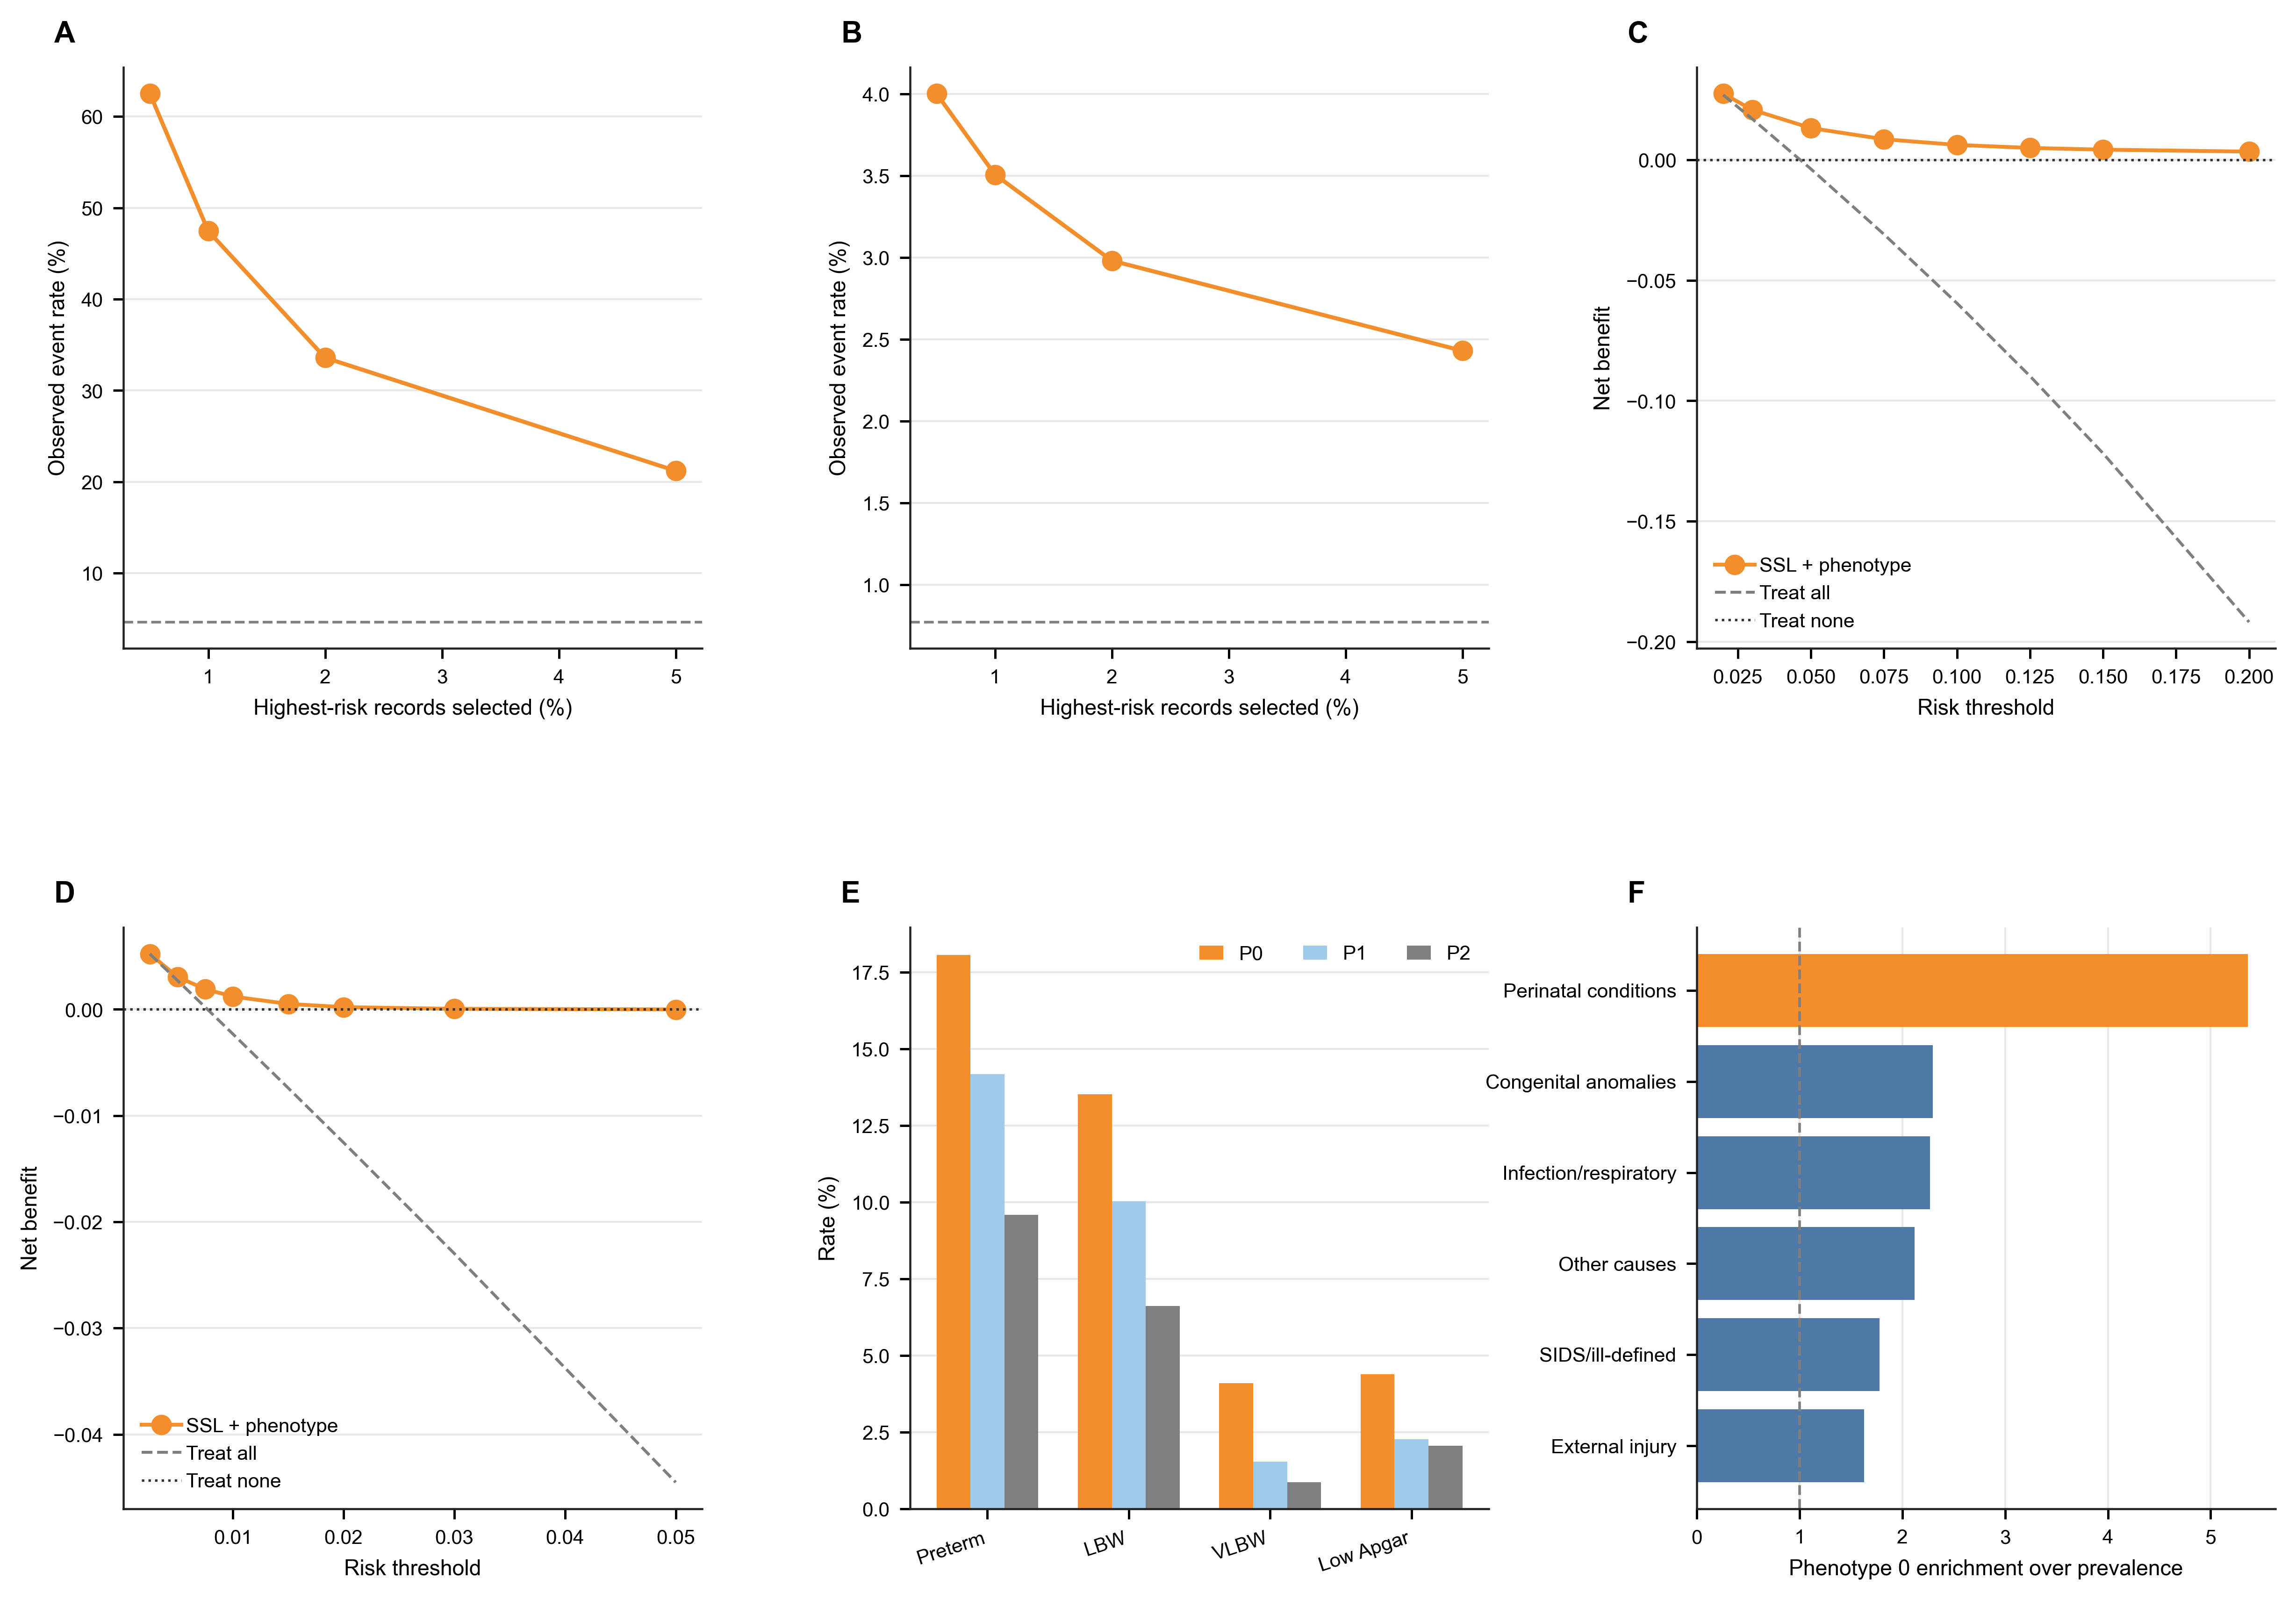
\includegraphics[width=\textwidth]{Figure_5_clinical_utility_interpretability.png}
\caption{\textbf{Clinical utility and phenotype interpretation.} \textbf{A,} Observed severe neonatal outcome event rate among the highest-risk 0.5\%, 1\%, 2\%, and 5\% of full-year 2024 test records ranked by the SSL plus phenotype score. \textbf{B,} Observed maternal core morbidity event rate among the same top-risk fractions. Dashed lines indicate full-year 2024 endpoint prevalence. \textbf{C,} Decision-curve analysis for severe neonatal outcome. \textbf{D,} Decision-curve analysis for maternal core morbidity. \textbf{E,} Birth-status profile by full-year 2024 phenotype assignment, including preterm birth, low birthweight, very low birthweight, and low 5-minute Apgar. \textbf{F,} Cause-specific infant death enrichment in the predefined linked-cohort high-risk phenotype 0. The dashed line indicates no enrichment over baseline prevalence.}
\label{fig5}
\end{figure}

\subsection{Full-scale SSL and linked severe-endpoint transfer analysis}\label{subsec:linked-results}

Full-scale pretraining materially improved reconstruction performance compared with the sampled prototype (Figure~\ref{fig6}A). The 2023 development reconstruction loss decreased from 0.284 in the 140,000-record prototype to 0.186 after streaming pretraining on all 26,345,765 training-period records. This supports the feasibility of scaling masked tabular SSL to national birth-registry size using a reproducible public-data workflow, although the lower reconstruction loss did not translate into improved downstream AUPRC beyond all-input LightGBM.

The full-year incremental LightGBM experiment clarified the predictive role of the SSL representation (Figure~\ref{fig6}B). For maternal morbidity, all-input LightGBM achieved AUPRC 0.0234, SSL embeddings alone achieved 0.0170, and all inputs plus SSL embeddings achieved 0.0230. For severe neonatal outcome, all-input LightGBM achieved AUPRC 0.3009, SSL embeddings alone achieved 0.2184, and all inputs plus SSL embeddings achieved 0.3008. Thus, full-scale SSL embeddings carried clinically relevant information but did not add consistent predictive improvement beyond all original leakage-controlled inputs.

Fixed phenotypes transferred to the linked birth/infant death cohort as a label-free risk-enrichment signal, but the supervised transfer baseline was stronger (Figure~\ref{fig6}C--D). In 3,596,017 linked 2023 births, infant death occurred in 19,743 records (0.549\%). The predefined high-risk phenotype 0 contained 164,651 births (4.58\%) and had an infant death rate of 2.021\% (95\% CI, 1.956--2.086), compared with 0.668\% in phenotype 1 and 0.299\% in phenotype 2. Phenotype 0 enriched infant death 3.68-fold over prevalence, neonatal death before 28 days 4.64-fold, early neonatal death before 7 days 5.07-fold, and postneonatal death 1.88-fold. At the same 4.58\% linked-cohort fraction, a transferred all-input LightGBM severe-neonatal score captured 49.09\% of infant deaths with an infant death rate of 5.886\% and 10.72-fold enrichment over prevalence, compared with 16.85\% capture by phenotype 0. Thus, the linked analysis supports phenotype transfer as descriptive representation evidence, not superiority over a supervised severe-risk score.

\begin{table}[!htbp]
\caption{\textbf{Linked infant-death transfer benchmark.}}
\label{tab:linked-transfer}
\centering
\scriptsize
\setlength{\tabcolsep}{3pt}
\begin{tabular*}{\textwidth}{@{\extracolsep{\fill}}lcccc@{}}
\toprule
Selection rule & Selected births & Death rate & Enrichment & Deaths captured \\
\midrule
Phenotype 0 & 164,651 (4.58\%) & 2.021\% & 3.68$\times$ & 16.85\% \\
LightGBM top 1\% & 35,960 (1.00\%) & 22.511\% & 41.00$\times$ & 41.00\% \\
LightGBM top 4.58\% & 164,651 (4.58\%) & 5.886\% & 10.72$\times$ & 49.09\% \\
LightGBM top 5\% & 179,801 (5.00\%) & 5.466\% & 9.96$\times$ & 49.78\% \\
\bottomrule
\end{tabular*}
\end{table}

In descriptive adjusted logistic models, phenotype 0 remained associated with infant death compared with phenotype 2. The maternal-registry adjusted odds ratio was 3.41 (95\% CI, 3.22--3.62) for infant death, 3.13 (95\% CI, 2.92--3.35) for neonatal death before 28 days, and 3.11 (95\% CI, 2.88--3.34) for early neonatal death before 7 days. After additional adjustment for gestational age and birthweight, these associations were attenuated but persisted for infant death (odds ratio, 1.94; 95\% CI, 1.81--2.07), neonatal death before 28 days (odds ratio, 1.61; 95\% CI, 1.48--1.74), and early neonatal death before 7 days (odds ratio, 1.95; 95\% CI, 1.79--2.13). These adjusted models were treated as descriptive sensitivity analyses, not causal estimates; the gestational-age and birthweight adjustments in particular may partially condition on variables that lie on the causal pathway from maternal-pregnancy vulnerability to infant death.

\begin{figure}[!htbp]
\centering
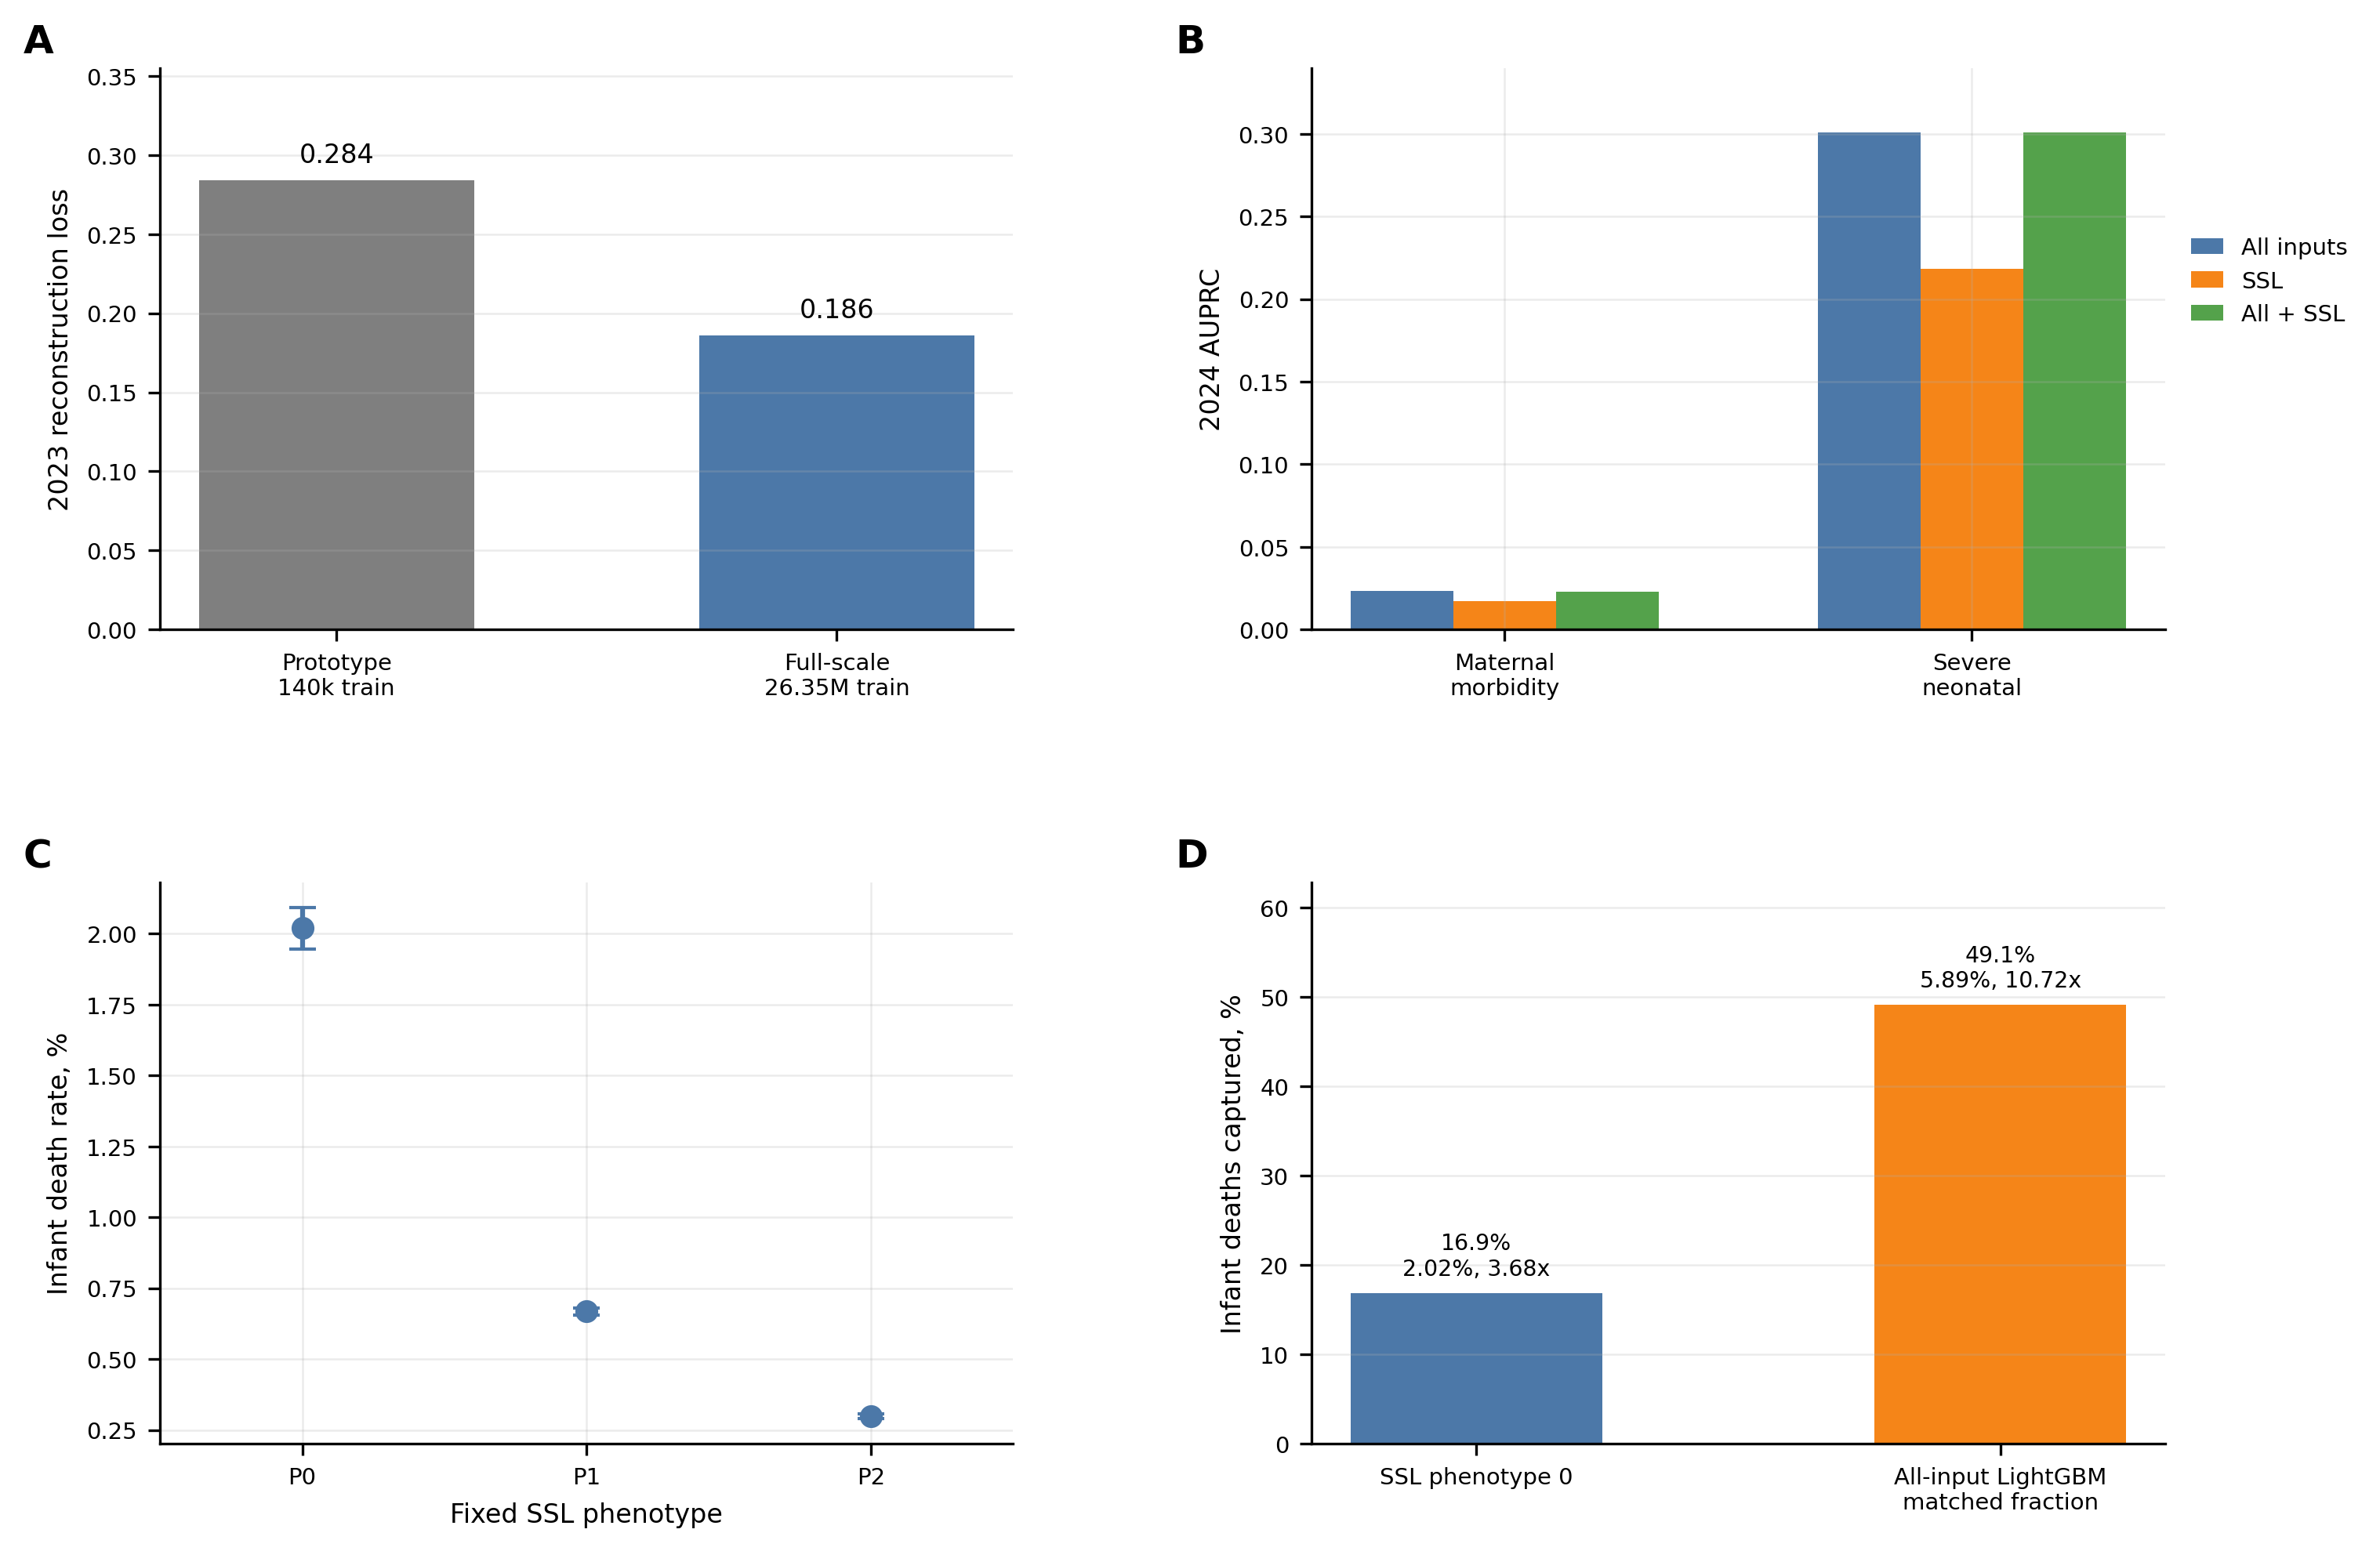
\includegraphics[width=\textwidth]{Figure_6_fullscale_linked_validation.png}
\caption{\textbf{Full-scale SSL pretraining, predictive increment testing, and linked severe-endpoint transfer analysis.} \textbf{A,} Development reconstruction loss for the sampled prototype and full-scale SSL pretraining run. Full-scale pretraining used all 26.35 million 2016--2022 records. \textbf{B,} Incremental LightGBM comparison on the full 3,638,436-record 2024 temporal test year. SSL embeddings carried risk signal but did not materially improve AUPRC when added to all leakage-controlled supervised inputs. \textbf{C,} Infant death rate in the 2023 linked birth/infant death cohort after assigning fixed SSL phenotypes learned from 2023 Natality development embeddings. Error bars show bootstrap 95\% confidence intervals. \textbf{D,} Matched-fraction transfer benchmark comparing infant deaths captured by the predefined high-risk phenotype 0 with those captured by a transferred all-input LightGBM severe-neonatal score at the same 4.58\% cohort fraction. Text annotations show event capture, selected-stratum infant death rate, and enrichment over baseline prevalence.}
\label{fig6}
\end{figure}

\subsection{Independent SINASC registry stress-test}\label{subsec:sinasc-results}

The independent SINASC stress-test extended the analysis beyond the U.S. public-use registry while keeping the interpretation deliberately conservative (Figure~\ref{fig7}). The separate SINASC encoder was trained and developed within 2023 records and evaluated once on the full 2024 SINASC test year. The 2024 severe birth-status endpoint had 90,268 events among 2,389,311 evaluable births (3.778\%), and the broad birth-status endpoint had 409,090 events (17.122\%).

Overlap-input LightGBM remained the strongest pure predictor in SINASC. For severe birth-status outcome, LightGBM achieved AUROC 0.676, AUPRC 0.132, AUPRC enrichment over prevalence of 3.48-fold, and top 1\% enrichment of 8.05-fold. SSL embeddings retained risk-enrichment signal but were weaker than LightGBM for pure prediction: SSL embedding logistic regression achieved AUROC 0.673, AUPRC 0.107, AUPRC enrichment of 2.83-fold, and top 1\% enrichment of 6.06-fold. SSL plus phenotype logistic regression was similar (AUPRC, 0.107; top 1\% enrichment, 6.03-fold), while phenotype-only prediction was weak (AUPRC enrichment, 1.05-fold). For broad birth-status outcome, LightGBM achieved AUPRC 0.378 and top 1\% enrichment of 4.93-fold, while SSL embeddings achieved AUPRC 0.341 and top 1\% enrichment of 4.43-fold. The phenotype risk ordering observed in U.S. data did not replicate cleanly in SINASC: 2024 severe birth-status rates were overlapping and non-monotonic across phenotypes 0, 1, and 2 (4.20\%, 3.45\%, and 4.01\%). These results support transportability of the analytic workflow across public birth registries, but not transportability of the fixed U.S. encoder or a universal phenotype labeling scheme.

\begin{figure}[!htbp]
\centering
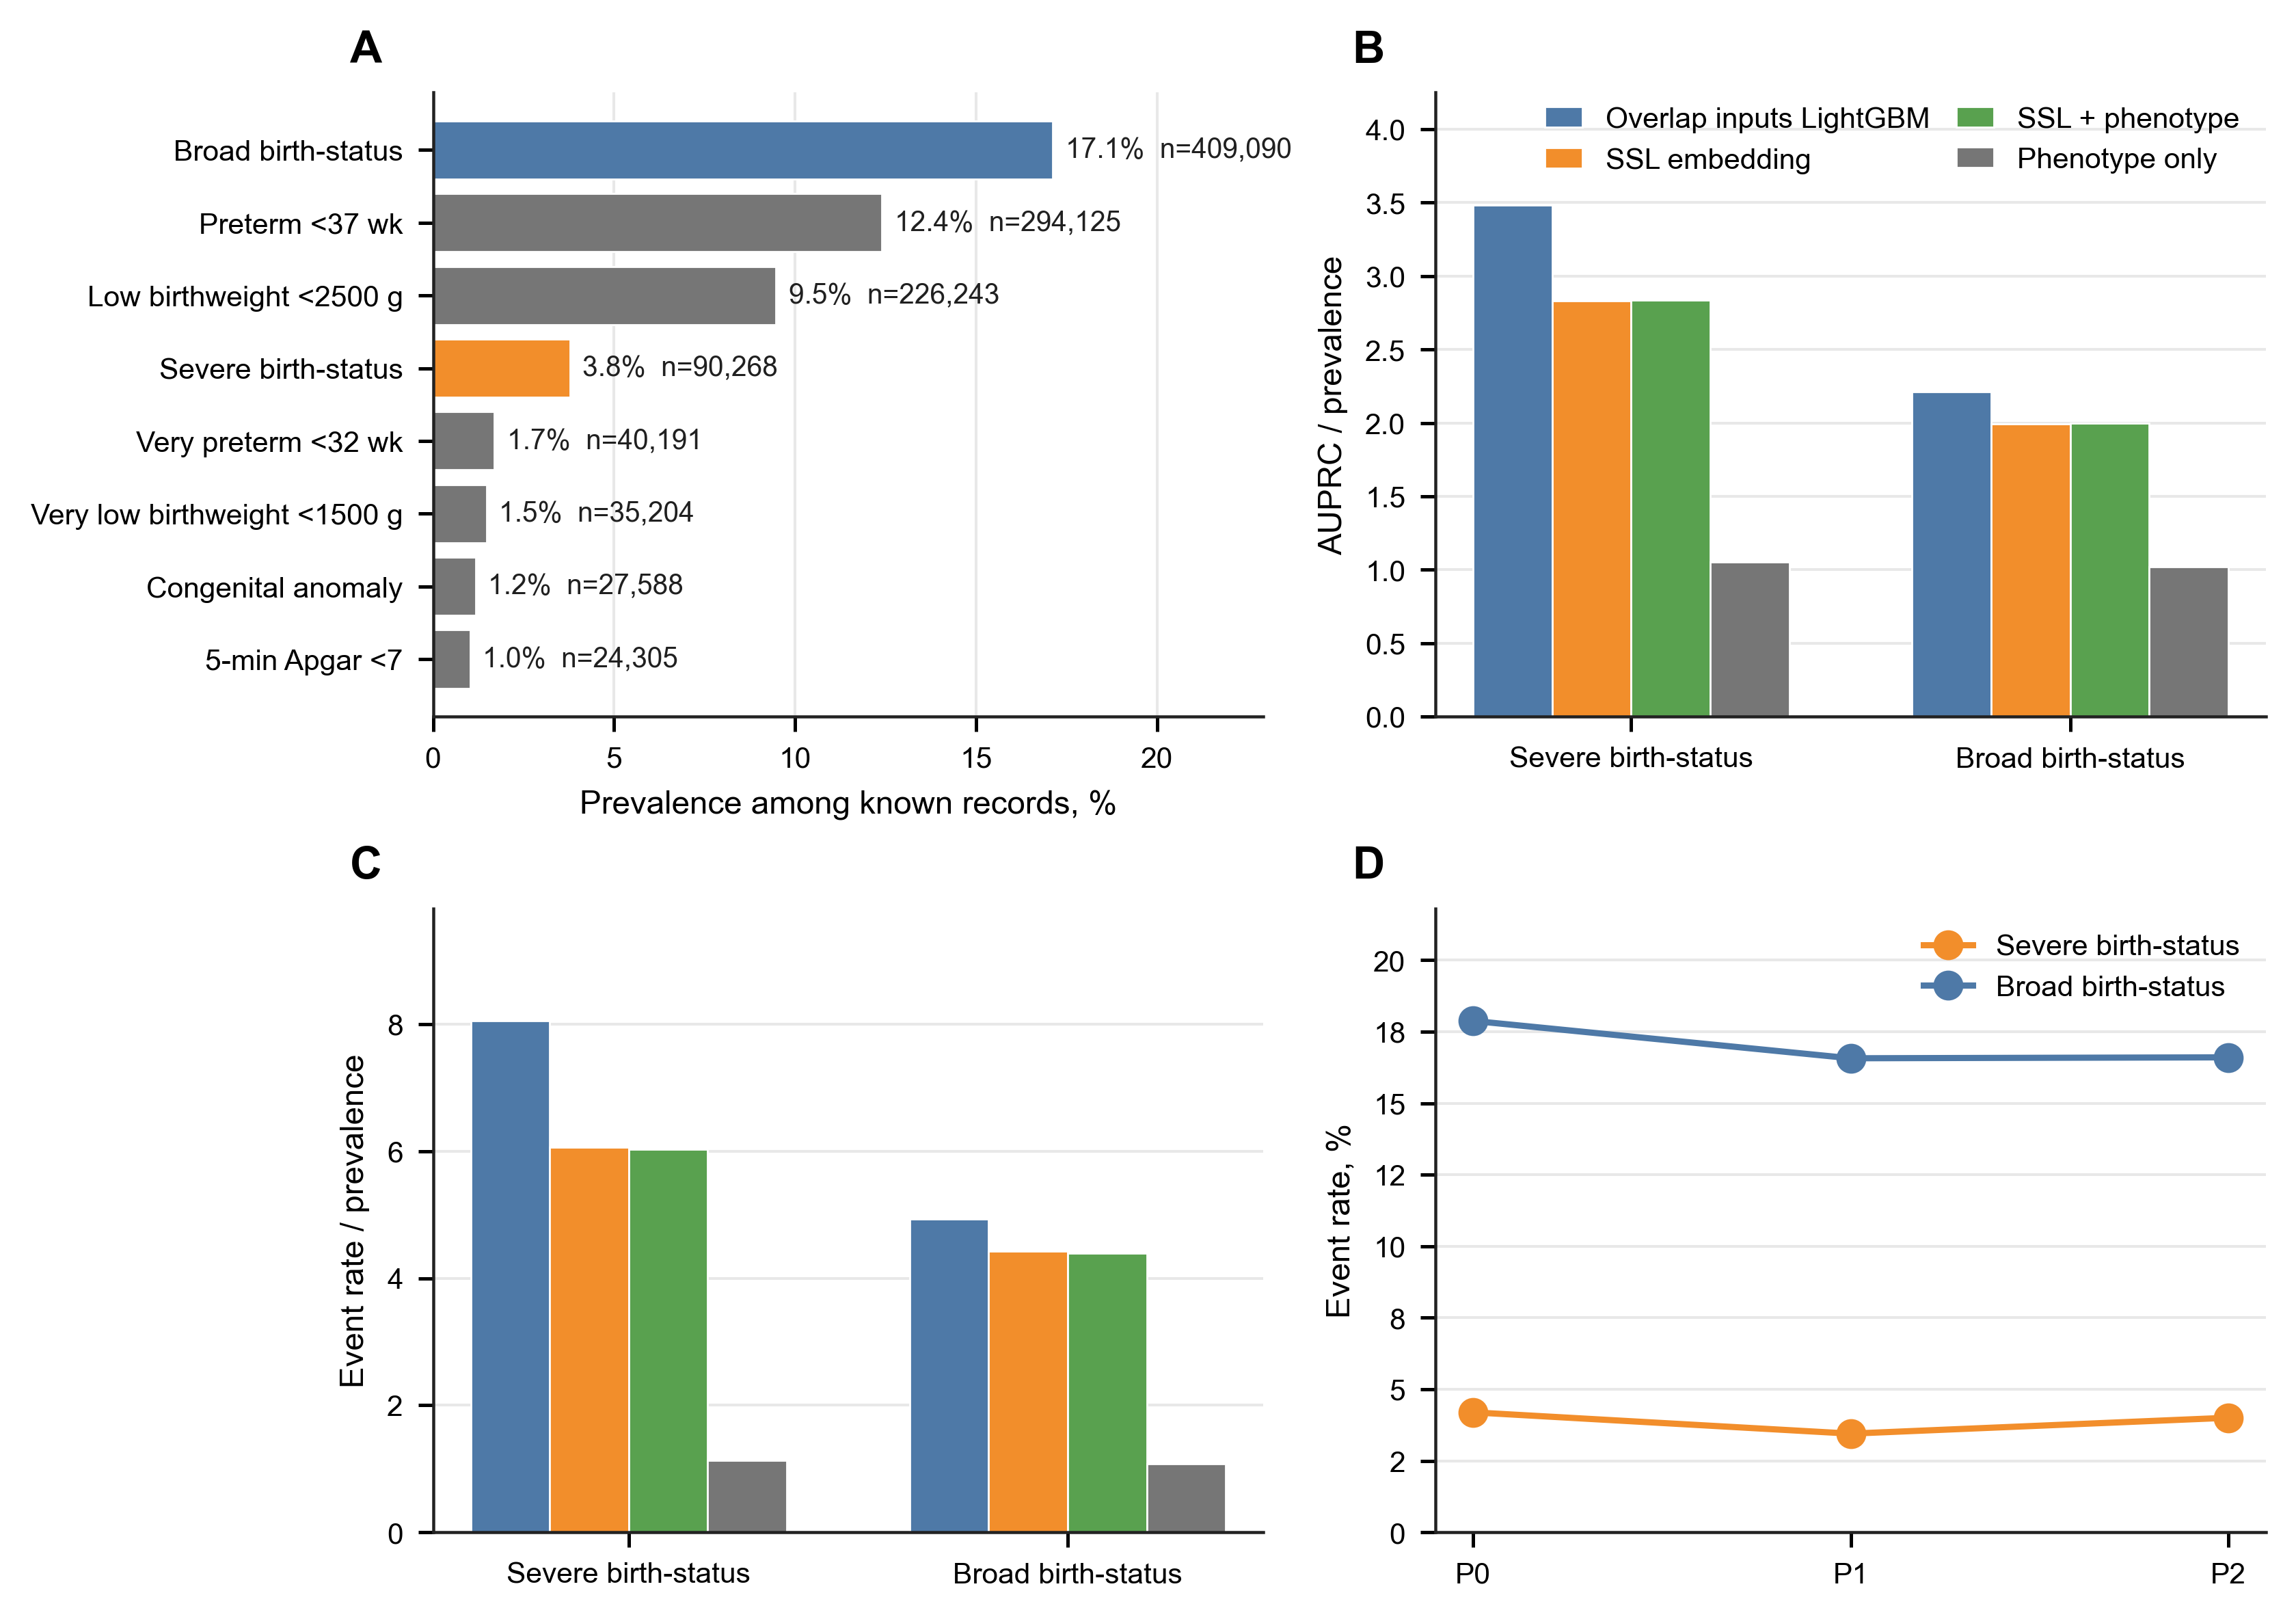
\includegraphics[width=\textwidth]{Figure_7_sinasc_registry_stress_test.png}
\caption{\textbf{Independent SINASC public-registry stress-test.} \textbf{A,} 2024 SINASC endpoint burden across harmonized birth-status outcomes and component endpoints. Bars show event prevalence among records with known outcome status, with event counts annotated at the bar end. \textbf{B,} AUPRC enrichment over outcome prevalence for severe and broad SINASC birth-status endpoints. \textbf{C,} Top 1\% risk enrichment for the same endpoints. \textbf{D,} Severe and broad birth-status rates by fixed SINASC phenotype in the 2024 test year. Overlap-input LightGBM remained the strongest pure predictor, whereas SSL embeddings retained risk-enrichment signal and phenotype-only prediction was weak.}
\label{fig7}
\end{figure}

\section{Discussion}\label{sec:discussion}

This study shows that full-scale masked tabular SSL can learn stable maternal comorbidity representations from public national birth records. In a calendar-time design using U.S. Natality data from 2016 through 2024, SSL embeddings supported reproducible phenotype discovery and risk enrichment above baseline prevalence for maternal and neonatal adverse outcomes. The linked birth/infant death analysis further showed that a fixed high-risk phenotype transferred to a severe mortality endpoint, but a transferred supervised all-input score provided substantially stronger mortality enrichment. A separately trained SINASC analysis showed that the workflow could be rebuilt in an independent public birth registry, although the U.S. phenotype risk ordering did not replicate as a universal taxonomy. The most defensible interpretation is not that SSL replaces supervised prediction, but that SSL adds a reproducible representation-learning and phenotype-description layer to public obstetric data.

The study should be interpreted alongside, rather than as a substitute for, EHR trajectory modeling. Prior EHR studies in preeclampsia and patient-timeline foundation models benefit from richer longitudinal information, repeated measurements, medications, diagnoses, and institution-level validation \cite{li2022preeclampsia_emr,yang2025preeclampsia_delivery,kraljevic2024foresight,yang2023transformehr,guo2024shared_ehr_foundation}. Our contribution is different: a transparent public-use registry workflow with calendar-time evaluation, strong supervised baselines, phenotype stability checks, calibration, top-risk enrichment, decision curves, subgroup screening, and source-data tables that can be independently scrutinized. This public-data framing is less clinically granular than private EHR work but more reproducible for external researchers.

The SINASC stress-test strengthens the reproducibility argument while also defining its boundary. Because Brazil SINASC lacks several U.S. Natality feature families, it would be misleading to apply the U.S. encoder directly and call the result external clinical validation. We therefore rebuilt the harmonized matrix and trained a separate SSL encoder under a 2023-to-2024 temporal split. This design showed that masked tabular representation learning and risk-enrichment evaluation were feasible in a distinct national registry, but the fixed SINASC phenotypes showed weaker outcome separation than the U.S. linked-infant-death phenotypes. The result is a workflow transport signal, not evidence of a universal maternal comorbidity phenotype taxonomy.

The full-year temporal comparison is important for interpreting the results. All-input LightGBM remained the strongest pure predictor for both primary endpoints, and adding SSL embeddings to all original supervised inputs did not materially improve AUPRC in the full 2024 test year. SSL embeddings were also evaluated within LightGBM, which partly separates representation content from the downstream model family; nevertheless, we did not interpret the logistic SSL models as direct competitors to all-input LightGBM. The findings are consistent with benchmark evidence that tree-based methods remain difficult to surpass on many tabular prediction tasks \cite{grinsztajn2022tree}. They are also expected from the learning objective: supervised models are directly optimized for the endpoint, whereas the SSL encoder was trained to reconstruct input structure. The linked infant-death transfer baseline reinforced this boundary, because the supervised severe-neonatal score enriched infant death more strongly than the fixed SSL phenotype at the same selected fraction. The value of SSL was therefore not predictive superiority, but the ability to produce stable latent representation summaries and clinically interpretable risk-enrichment strata that can be audited independently of any one supervised label.

The clinical-utility analyses make the same point from a decision perspective. The top-risk and decision-curve results indicate that SSL plus phenotype can enrich adverse outcomes above baseline prevalence, especially for severe neonatal outcome, but the absolute net-benefit gains were modest and weaker than strong supervised prediction. This may still be useful for retrospective prioritization, cohort enrichment, and quality-improvement hypothesis generation. It should not be over-read as evidence that the model can diagnose individual outcomes, guide intrapartum decisions, or be deployed without prospective validation. The birth-status and cause-specific infant death analyses were consistent with expected clinical gradients, because the high-risk phenotype was associated with shorter gestation, lower birthweight, low Apgar, and disproportionate enrichment of perinatal-condition deaths. These are descriptive associations, not causal explanations.

The phenotype results suggest that public-use maternal and pregnancy variables contain reproducible latent structure. Phenotype 0 was a smaller group enriched for maternal core morbidity, severe neonatal outcome, linked infant death, preterm birth, low birthweight, very low birthweight, and low 5-minute Apgar. Its prototype profile differed across BMI, prenatal care, obstetric history, smoking, selected infection-related variables, and missingness patterns. The cause-specific linked mortality pattern was strongest for perinatal-condition deaths, which is consistent with a maternal/pregnancy vulnerability profile rather than a nonspecific artifact. However, the analysis is observational and registry-based. Because missingness indicators were part of the input matrix, the phenotypes may partly capture documentation completeness, reporting practices, or care-access patterns in addition to clinical comorbidity structure. The phenotypes should not be interpreted as causal disease subtypes or direct clinical categories without additional validation.

The calibration analysis addresses an important translational issue. Raw model scores, whether from SSL-derived logistic models or supervised models, should not be treated as absolute clinical probabilities. Platt recalibration was used to place downstream scores on a more interpretable retrospective risk scale. However, calibration in one calendar year does not guarantee calibration in another health system, coding environment, or prospective workflow. This supports potential use in risk enrichment, cohort triage, or retrospective public health analysis, but not immediate deployment as a clinical decision system.

The PCA sensitivity analysis provides additional insight into the SSL representation and clarifies a boundary of the phenotype analysis. Severe neonatal outcome prediction degraded substantially when embeddings were reduced to five or ten principal components, whereas 32 components retained much of the full embedding signal. The three-phenotype solution was fit in a 16-component PCA space selected for reproducible unsupervised partitioning rather than downstream prediction. Therefore, the phenotype labels should be viewed as stable representation summaries, not as a complete compression of all outcome-relevant SSL information. This also explains why phenotype-only prediction was weak and motivates future work on lower-dimensional latent summaries selected jointly for stability, interpretability, and clinical utility.

This study has several limitations. First, Natality public-use records are registry data and do not include laboratory values, medication exposures, fetal monitoring waveforms, longitudinal visits, imaging, free text, or full clinical adjudication. The work therefore does not claim the same trajectory resolution as EHR-based pregnancy journey studies. Second, registry-defined maternal morbidity is known to be under-ascertained and variably reported in vital records; this measurement ceiling likely contributed to the low absolute maternal AUPRC even for the strongest supervised model. Third, registry variables and outcomes can be affected by differential coding, documentation, and missingness across states, institutions, and patient groups. Missingness indicators may improve prediction while also encoding health-care access or reporting processes, so phenotype profiles should be interpreted clinically but cautiously. Fourth, some birth-certificate predictors, including selected infections and risk-factor fields, may be finalized at delivery rather than captured prospectively at a prenatal encounter. We therefore frame the models as registry risk-enrichment analyses, not real-time antepartum prediction tools. Fifth, some predictors, particularly gestational hypertensive disorders and eclampsia, sit close to the maternal morbidity pathway. They were not components of the primary maternal endpoint, but their inclusion may represent near-outcome conditioning for maternal risk modeling. Sixth, although development, calibration, phenotype discovery, and final 2024 embedding evaluation were performed at full calendar-year scale, the stability resampling analysis used a 500,000-record cap per resample for computational tractability and should be interpreted as a large-sample stability check rather than exhaustive reclustering of every resample. Seventh, the linked infant death analysis should not be interpreted as independent external clinical validation. It is a linked severe-endpoint transfer analysis within the CDC/NCHS public-use ecosystem: the endpoint is more severe and was not used for SSL training or phenotype discovery, but the data source remains a national vital-statistics registry rather than an independent hospital or health-system registry. Eighth, the SINASC analysis was an independent public-registry stress-test, but it was not direct external validation of the U.S. model. Endpoint definitions and input features differed, the SINASC encoder and phenotypes were trained separately, and the U.S.-like phenotype risk ordering did not replicate cleanly. Ninth, the adjusted linked infant death models are descriptive. Adjustment for gestational age and birthweight helps test attenuation of the phenotype association, but these variables may be downstream of maternal and pregnancy risk and should not be treated as a causal adjustment set or as pre-delivery deployment inputs. Tenth, phenotype labels were derived from k-means clustering and should be considered reproducible partitions of a continuous embedding rather than natural disease classes. We did not include a full raw-input k-means phenotype baseline or a complete raw-versus-SSL by logistic-versus-gradient-boosting model-family grid, so the study cannot prove that SSL clustering is superior to every simpler input-space clustering strategy. Eleventh, many endpoints, metrics, thresholds, subgroup strata, and sensitivity analyses were examined; confidence intervals should therefore be interpreted as uncertainty summaries rather than multiplicity-adjusted confirmatory tests. Twelfth, subgroup checks were limited to available public-use variables and are not a comprehensive fairness audit. Finally, bootstrap confidence intervals quantify within-sample sampling uncertainty in very large samples; they do not capture dominant sources of uncertainty such as coding drift, temporal drift, model initialization, or absence of prospective clinical validation.

Future work should evaluate representation transport in independent data sources, incorporate richer electronic health record or physiologic data where available, and test whether SSL-derived phenotypes improve clinical workflow design, subgroup monitoring, or targeted quality-improvement strategies. Any future clinical use would require prospective validation, local recalibration, predefined action thresholds linked to feasible interventions, safety monitoring, and evaluation of fairness across maternal demographic and obstetric subgroups.

\section{Conclusions}\label{sec:conclusions}

Full-scale masked tabular SSL on U.S. Natality public-use records produced stable maternal comorbidity embeddings and clinically profiled latent phenotypes associated with adverse maternal, neonatal, and linked infant death outcomes. In full-year temporal testing, SSL-derived models did not outperform all-input LightGBM for pure prediction, and a supervised severe-neonatal score transferred more strongly than phenotype 0 to linked infant death. Fixed phenotypes nevertheless provided reproducible representation summaries and risk enrichment above baseline prevalence. A separately trained SINASC analysis showed that the workflow could be rebuilt in an independent public birth registry, although it did not establish fixed-model clinical transportability or a universal phenotype taxonomy. The approach is best viewed as a transparent public-data representation-learning framework for obstetric phenotype discovery, severe-risk enrichment, cross-registry stress-testing, and hypothesis generation rather than a bedside prediction model.

\backmatter

\section*{Abbreviations}

ART, assisted reproductive technology; AUPRC, area under the precision--recall curve; AUROC, area under the receiver operating characteristic curve; CDC/NCHS, Centers for Disease Control and Prevention/National Center for Health Statistics; EHR, electronic health record; ICD-10, International Classification of Diseases, Tenth Revision; LightGBM, light gradient boosting machine; NICU, neonatal intensive care unit; PCA, principal component analysis; SINASC, Sistema de Informacao sobre Nascidos Vivos; SSL, self-supervised learning.

\section*{Additional files}

\textbf{Additional file 1: Source-data tables and reproducibility scripts.} ZIP archive containing source-data tables supporting the main figures and key manuscript claims, selected analysis scripts, figure-building scripts, configuration files, small fitted model artifacts, and license information. The tables include model metrics, bootstrap confidence intervals, full-year 2024 embedding evaluation outputs, linked infant death phenotype rates, supervised linked infant death transfer baseline, descriptive adjusted linked infant death logistic models, cause-specific linked infant death profiles, phenotype profiles, PCA sensitivity, top-risk utility summaries, decision-curve outputs, subgroup metrics, SINASC variable crosswalk tables, SINASC harmonized outcome prevalence, and SINASC stress-test metrics. No individual-level CDC/NCHS or SINASC public-use records are redistributed.

\textbf{Additional file 2: Reporting checklist mapping.} STROBE and TRIPOD+AI item-to-section mapping for the observational registry analysis, prediction-model components, temporal validation, calibration, data availability, and limitations.

\section*{Declarations}

\subsection*{Acknowledgements}

Not applicable.

\subsection*{Ethics approval and consent to participate}

Ethics approval was not required for this study because all analyses used publicly available de-identified public-use records from CDC/NCHS and Brazil OpenDataSUS. The analysis did not involve direct contact with participants, intervention, or access to restricted individual-level clinical records. Informed consent was not required for this secondary analysis of de-identified public-use data.

\subsection*{Consent for publication}

Not applicable.

\subsection*{Availability of data and materials}

The raw Natality public-use files and user guides are available from CDC/NCHS public-use data portals, including Vital Statistics Online Data Access and the 2024 Natality public-use file documentation \cite{nchs_vitalstats_online,nchs_natality_2024_userguide}. The linked birth/infant death public-use file documentation is available from CDC/NCHS \cite{nchs_linked_2024_userguide}. The raw SINASC public-use files and structure dictionary are available from Brazil OpenDataSUS \cite{opendatasus_sinasc,sinasc_structure_dictionary}. Processed analytic data were generated from public-use records using the scripts provided in Additional file 1. Individual-level CDC/NCHS and SINASC public-use records are not redistributed.

\subsection*{Competing interests}

The authors declare no competing interests.

\subsection*{Funding}

No external funding was received for this study.

\subsection*{Authors' contributions}

F.Y., Q.Y., and M.W. contributed equally to data processing, analysis, figure preparation, and manuscript drafting. F.L. conceptualized and supervised the study, reviewed the analysis, and revised the manuscript. All authors read and approved the final manuscript.

\subsection*{Code availability}

Source scripts, generated source-data tables, figure-building scripts, the final masked-tabular SSL checkpoint, fitted preprocessing metadata, phenotype centroid file, and the MIT license are provided as Additional file 1 and in the public GitHub repository at \url{https://github.com/Luciky-Leo/natality-comorbidity-ssl}. The versioned archival release is available from Zenodo at \url{https://doi.org/10.5281/zenodo.20482195}. The scripts use the official public-use sources described above; raw individual-level public-use records are not redistributed. The trained supervised LightGBM transfer model was not redistributed because it can be regenerated from the public-use files using the provided script and deterministic split identifiers.

\bibliography{references}

\end{document}
